\documentclass[11pt,a4paper]{article}

% ---------------------------------------------------------------- packages
\usepackage[utf8]{inputenc}
\usepackage[T1]{fontenc}
\usepackage{mathptmx}
\usepackage[scaled=.90]{helvet}
\usepackage{courier}
\usepackage[a4paper,margin=2.5cm]{geometry}
\usepackage{microtype}
\usepackage{setspace}
\usepackage{amsmath,amssymb,amsthm}
\usepackage{graphicx}
\usepackage{booktabs,array,tabularx,multirow,colortbl}
\usepackage{xcolor}
\usepackage{caption}
\usepackage{enumitem}
\usepackage{placeins}
\usepackage{fancyhdr}
\usepackage[ruled,vlined,linesnumbered,noend]{algorithm2e}
\usepackage{tikz}
\usetikzlibrary{positioning,arrows.meta,shapes.geometric,fit}
\usepackage[colorlinks=true,linkcolor=blue!50!black,citecolor=blue!50!black,urlcolor=blue!50!black]{hyperref}

\linespread{1.08}
\setlength{\parskip}{0.4em}
\setlength{\parindent}{0pt}
\captionsetup{font=small,labelfont=bf}
\SetKwComment{Comment}{$\triangleright$\ }{}
\SetCommentSty{textit}
\renewcommand{\arraystretch}{1.12}

\pagestyle{fancy}
\fancyhf{}
\fancyhead[L]{\small Learning-Path Optimization as a 0/1 Knapsack Problem}
\fancyhead[R]{\small Design and Complexity of Algorithms}
\fancyfoot[C]{\small\thepage}
\renewcommand{\headrulewidth}{0.3pt}

% ---------------------------------------------------------------- theorem environments
\theoremstyle{plain}
\newtheorem{theorem}{Theorem}
\newtheorem{lemma}[theorem]{Lemma}
\newtheorem{proposition}[theorem]{Proposition}
\theoremstyle{definition}
\newtheorem{definition}{Definition}
\theoremstyle{remark}
\newtheorem{remark}{Remark}

% ---------------------------------------------------------------- shortcuts
\renewcommand{\_}{\textunderscore\hspace{0pt}}  % allow line breaks after underscores in file names
\newcommand{\code}[1]{\texttt{#1}}
\newcommand{\OPT}{\mathrm{OPT}}
\newcommand{\bigO}{\mathcal{O}}

\begin{document}

% ================================================================= COVER
\begin{titlepage}
\centering
{\large Universidade de Bras\'ilia (UnB)\par}
{\large Departamento de Ci\^encia da Computa\c{c}\~ao\par}
\vspace{0.6cm}
{\normalsize Design and Complexity of Algorithms\par}
{\normalsize Professor Marcelo Antonio Marotta\par}
{\normalsize Final Project\par}
\vspace{2.2cm}
{\LARGE\bfseries Learning-Path Optimization as a 0/1 Knapsack Problem\par}
\vspace{0.4cm}
{\Large Dynamic Programming versus the Exhaustive DFS of RUTICO and Greedy Selection\par}
\vspace{1.4cm}
\begin{tabular}{rl}
\textbf{Problem:} & Selecting the set of learning modules that maximizes the\\
& learning score within a study-time budget\\
& (0/1 Knapsack Problem)\\[4pt]
\textbf{Article studied:} & RUTICO: Recommending Successful Learning Paths\\
& Under Time Constraints (UMAP 2017)\\[4pt]
\textbf{Algorithms:} & Exhaustive DFS (authors), Dynamic Programming\\
& (proposal), Greedy by score/time ratio (comparison),\\
& plus Branch and Bound, Meet-in-the-Middle and FPTAS\\
\end{tabular}
\vspace{1.6cm}

{\large\bfseries Group members\par}
\vspace{0.3cm}
\begin{tabular}{ll}
{[Member Name 1]} & {[Student ID 1]}\\
{[Member Name 2]} & {[Student ID 2]}\\
{[Member Name 3]} & {[Student ID 3]}\\
{[Member Name 4]} & {[Student ID 4]}\\
\end{tabular}
\vfill
{\normalsize Bras\'ilia, October 2026\par}
\end{titlepage}

% ================================================================= ABSTRACT
\pagenumbering{roman}
\begin{abstract}
\noindent Choosing which learning modules a student should study within a limited amount of time is a combinatorial optimization problem that arises in e-learning recommender systems. We model it as the 0/1 Knapsack Problem and study it through the article \emph{RUTICO: Recommending Successful Learning Paths Under Time Constraints}, whose solution enumerates the feasible paths of a course graph with a depth-first search (DFS). We analyze the design and the complexity of three algorithmic strategies: the exhaustive DFS with time pruning used by the authors, a Dynamic Programming (DP) algorithm that we propose, and a greedy heuristic based on the score/time ratio. Three further algorithms (Branch and Bound, Meet-in-the-Middle and an FPTAS) are used as additional points of comparison. We prove the correctness and derive the best-, worst- and average-case behavior of each algorithm, and we validate the analysis with a hand-written Python implementation and with experiments that count elementary operations, so that conclusions do not depend on the hardware. The DFS generates exactly $2^{n+1}-1$ nodes in its worst case, whereas the DP performs exactly $n(T+1)$ operations on any instance and is pseudo-polynomial; the greedy heuristic is fast but loses up to 54.5\% of the optimal score on our small random instances and 99.8\% on an adversarial instance. We show that DP is the most suitable algorithm for the learning-path scenario, since it is exact, has a predictable cost, and the budget $T$ is small in practice, and we discuss the regimes in which the alternative algorithms win. All code, data and plots are available in the accompanying source package.

\vspace{0.4cm}
\noindent\textbf{Keywords:} knapsack problem, dynamic programming, depth-first search, greedy algorithms, pseudo-polynomial time, learning paths, algorithm analysis.
\end{abstract}

\clearpage
\tableofcontents
\clearpage
\pagenumbering{arabic}

\section{Introduction}\label{sec:intro}

\subsection{Motivation and problem statement}

Online learning environments offer far more material than any learner can study. A student who can dedicate only a few hours per week must therefore decide \emph{which} learning modules to take, and this decision directly affects how much is learned. Learning-path recommender systems address this decision by personalizing the sequence of learning activities that leads a learner toward a goal \cite{nabizadeh2020survey}. Among the limitations that such systems must respect, the available study time is one of the most concrete: modules take time, and the learner's time is finite.

The article studied in this project, \emph{RUTICO: Recommending Successful Learning Paths Under Time Constraints} \cite{nabizadeh2017rutico}, addresses exactly this situation. After locating the learner in the course graph, RUTICO uses a depth-first search (DFS) to find all possible paths that fit in the learner's time restriction and recommends the path with the maximum score. The article therefore poses a clear optimization problem (maximize a learning score under a time budget) and presents a clear solution (exhaustive DFS).

We isolate the combinatorial core of this problem. Each learning module $i \in \{1,\dots,n\}$ has an integer study time $w_i \ge 1$ and a non-negative score $v_i$ that quantifies the expected learning benefit; the learner has an integer time budget $T \ge 0$.

\begin{definition}[Learning-path selection problem]\label{def:lps}
Given $n$ modules with times $w_i$ and scores $v_i$ and a budget $T$, find a subset $S \subseteq \{1,\dots,n\}$ that maximizes $v(S)=\sum_{i\in S} v_i$ subject to $w(S)=\sum_{i\in S} w_i \le T$.
\end{definition}

Definition~\ref{def:lps} is the classical \emph{0/1 Knapsack Problem}: each module is taken entirely or not at all. In this formulation the modules are independent of each other. The course graph of the article additionally imposes prerequisites; ignoring them is a deliberate \emph{relaxation} that we state explicitly and discuss in Sections~\ref{sec:decisions} and~\ref{sec:conclusion}.

\subsection{Techniques and algorithms studied}

The assignment requires analyzing the algorithm created by the authors of the article, implementing it, and comparing it with at least one other approach from the literature. We therefore study three algorithms that play distinct roles, and three additional ones that broaden the comparison (Table~\ref{tab:roles}).

\begin{table}[h]
\centering
\caption{Roles of the algorithms and design techniques studied.}\label{tab:roles}
\footnotesize
\begin{tabularx}{\linewidth}{@{}p{2.5cm} p{3.9cm} X p{3.3cm}@{}}
\toprule
Role & Algorithm & Design technique & Source file\\
\midrule
Authors (article) & Exhaustive DFS with time pruning & Depth-first search with backtracking & \code{dfs.py}\\
Proposal & 0/1 Knapsack DP (table, vector, memoized) & Dynamic programming & \code{dp.py}\\
Comparison (mandatory) & Greedy by score/time ratio & Greedy strategy (and merge sort: divide and conquer) & \code{greedy.py}\\
Extra comparison & Branch and Bound & Implicit enumeration with bounding & \code{branch\_and\_bound.py}\\
Extra comparison & Meet-in-the-Middle & Divide and conquer on the input set & \code{meet\_in\_the\_middle.py}\\
Extra comparison & FPTAS & Value scaling + DP over the profit & \code{fptas.py}\\
Extension & DFS over the prerequisite graph & Graph search with backtracking & \code{graph\_dfs.py}\\
\bottomrule
\end{tabularx}
\end{table}

The central argument of the project is that these techniques are not unrelated. The DFS of the authors explores a decision tree with $2^n$ leaves in which many branches reach the same state; dynamic programming is, in essence, the same search with each state computed only once. This explains why DP is the natural proposal: it keeps the exactness of the exhaustive search and removes its exponential redundancy (Section~\ref{sec:design}).

\subsection{Contributions}

\begin{itemize}[leftmargin=1.4em,itemsep=2pt]
\item A formal model of the learning-path selection problem and its relation to the knapsack family, including the relaxation with respect to the article (Sections~\ref{sec:intro} and~\ref{sec:background}).
\item A design analysis that derives dynamic programming from the authors' DFS (Section~\ref{sec:design}).
\item Proofs of correctness and of best-, worst- and (empirical) average-case complexity for every algorithm, including approximation guarantees for the greedy variants and the FPTAS (Section~\ref{sec:complexity}).
\item A modular Python implementation written without algorithmic libraries, in which every algorithm returns a common result type with an operation counter (Section~\ref{sec:implementation}).
\item An experimental evaluation that validates correctness on more than one thousand random instances, measures growth rates in operations and in time, tests three families of instances with different correlation between time and score, and demonstrates the pseudo-polynomial behavior of DP (Section~\ref{sec:experiments}).
\item A discussion of why DP is the most suitable algorithm for this scenario, and of the regimes in which each alternative wins (Section~\ref{sec:discussion}).
\end{itemize}

\subsection{Organization of this report}

Section~\ref{sec:background} presents the theoretical background. Section~\ref{sec:design} covers the algorithm design (assignment item 1.1.1). Section~\ref{sec:implementation} describes the implementation, pseudocode and the test instance. Section~\ref{sec:complexity} contains the complexity analysis (item 1.1.2). Section~\ref{sec:experiments} reports the experiments, and Section~\ref{sec:discussion} discusses the results. Section~\ref{sec:members} lists the activities of each member, and Section~\ref{sec:conclusion} concludes the report with the main difficulties encountered.

\section{Theoretical Background}\label{sec:background}

This section presents the concepts on which the rest of the report relies. Each subsection ends by indicating the code module in which the concept materializes, so that the theory and the implementation can be read side by side (a summary is given in Table~\ref{tab:theory-code}).

\subsection{Learning-path optimization in e-learning}

A learning path is the implementation of a curriculum design: a set of learning activities that helps a user achieve particular learning goals. Because learners differ in their limitations, backgrounds and goals, personalizing these paths became a significant research task, and the survey of Nabizadeh et al.\ organizes the methods, the parameters used for personalization and the evaluation approaches of this area \cite{nabizadeh2020survey}. Available study time is one of the limitations a learner may have, and it is the one that RUTICO addresses directly \cite{nabizadeh2017rutico}: the system looks for paths whose total duration respects the learner's time restriction and whose score is maximal.

When modules have prerequisites, the feasible selections form a structure over a directed acyclic graph (DAG). The corresponding optimization problem is the \emph{precedence-constrained knapsack problem} (PCKP), in which a module can be adopted only if all its predecessors are in the knapsack \cite{samphaiboon2000}. PCKP is NP-hard because it contains the plain knapsack as the special case without precedence, and dynamic programming algorithms for it are known to solve small instances to optimality \cite{samphaiboon2000}. Ignoring prerequisites therefore yields a strictly simpler problem whose structure is completely understood, and which is the subject of this work. The graph search of RUTICO itself is represented in our code by \code{graph\_dfs.py}.

\subsection{The 0/1 knapsack problem}\label{sec:knapsack}

Definition~\ref{def:lps} can be written as the integer linear program
\begin{equation}
\max \sum_{i=1}^{n} v_i x_i \quad \text{s.t.}\quad \sum_{i=1}^{n} w_i x_i \le T,\quad x_i \in \{0,1\},
\label{eq:ilp}
\end{equation}
where $x_i=1$ means that module $i$ is selected. Without loss of generality we assume $w_i \le T$ for every module, since a module that does not fit alone can never be part of a solution.

\paragraph{Computational complexity.} The decision version of the problem (is there a subset with $v(S)\ge V$ and $w(S)\le T$?) is NP-complete; the knapsack problem is among the problems whose NP-completeness was established by Karp \cite{karp1972} and it is a standard example in the theory of NP-completeness \cite{garey1979}. No polynomial-time algorithm is known for it, but it is NP-hard only in the \emph{weak} sense: there are algorithms whose running time is polynomial in the \emph{numeric value} of the input, called pseudo-polynomial algorithms \cite{garey1979,kellerer2004}. The input of Definition~\ref{def:lps} is encoded with $\Theta\big(n \log(T+\max_i w_i+\max_i v_i)\big)$ bits, so a running time such as $\Theta(nT)$ is exponential in the number of bits used to write $T$, even though it is linear in the number $T$ itself. This distinction is the key to understanding both the efficiency of dynamic programming in practice and its limitation (Sections~\ref{sec:design} and~\ref{sec:experiments}). Despite its NP-hardness, many knapsack instances are easy for modern algorithms, and Pisinger studies which classes of instances remain hard \cite{pisinger2005}.

\paragraph{Fractional relaxation.} If modules could be taken partially ($x_i\in[0,1]$), the problem would be solved optimally by a greedy rule: sort the modules by decreasing ratio $v_i/w_i$ and take them in this order until the first module that does not fit, of which only a fraction is taken. This observation, due to Dantzig \cite{dantzig1957}, has two consequences that we exploit: it gives an upper bound on the 0/1 optimum (used by Branch and Bound), and it explains both why a ratio-based greedy is attractive and why it fails when items are indivisible.

\subsection{Algorithm design paradigms}

\subsubsection{Backtracking and depth-first search}

Backtracking systematically builds candidate solutions and abandons (prunes) a partial candidate as soon as it cannot lead to a feasible solution \cite{golomb1965}. It is implemented with a depth-first traversal of the \emph{decision tree}, in which each level corresponds to a decision (here: include or exclude one module) and each leaf to a complete selection. Depth-first search itself is a linear-time graph traversal \cite{tarjan1972,cormen2022}. A recursive implementation must \emph{restore} the state when it returns from a recursive call (the backtracking step), otherwise decisions of one branch leak into the other. For the knapsack, the tree has $2^n$ leaves; pruning the ``include'' branch whenever the time budget would be exceeded removes infeasible subtrees but does not change the exponential worst case. This is the technique of the authors' solution (\code{dfs.py}, \code{graph\_dfs.py}).

\subsubsection{Dynamic programming}

Dynamic programming, introduced by Bellman \cite{bellman1957}, solves an optimization problem by combining solutions of subproblems and is applicable when the problem has two properties \cite{cormen2022,kleinberg2006}:

\begin{itemize}[leftmargin=1.4em,itemsep=1pt]
\item \textbf{Optimal substructure:} an optimal solution contains optimal solutions of its subproblems (Bellman's principle of optimality).
\item \textbf{Overlapping subproblems:} the same subproblems are needed repeatedly, so computing each one once and reusing its value saves work.
\end{itemize}

There are two equivalent implementations. \emph{Bottom-up} fills a table in an order that guarantees that dependencies are ready; \emph{top-down} keeps the recursive formulation and caches results, a technique known as memoization, named after Michie's ``memo functions'' \cite{michie1968}. Both compute the same values; the top-down version computes only the states that are actually reachable, at the price of recursion overhead. When each row of the table depends only on the previous one, the table can be compressed into a single vector, reducing the space. Dynamic programming is the proposal of this project (\code{dp.py}: \code{dp\_table}, \code{dp\_vector}, \code{dp\_memoized}).

\subsubsection{Greedy strategy}

A greedy algorithm builds a solution by repeatedly making the locally best choice. It is correct when the problem has the greedy-choice property and optimal substructure \cite{cormen2022}; the fractional knapsack has it (Section~\ref{sec:knapsack}), the 0/1 knapsack does not. Applied to the 0/1 knapsack, the ratio-based greedy is fast but offers no optimality guarantee, and it can be arbitrarily bad (Proposition~\ref{prop:greedy-unbounded}). A simple modification, returning the better of the greedy solution and the best single module, guarantees at least half of the optimum \cite{kellerer2004} (Proposition~\ref{prop:greedy-half}). The greedy strategy is our mandatory comparison algorithm (\code{greedy.py}); it relies on a sort, which we implement as a merge sort (divide and conquer, \code{sorting.py}).

\subsubsection{Branch and Bound}

Branch and Bound, proposed by Land and Doig for discrete programming \cite{land1960}, explores the decision tree like the DFS but discards a subtree when an \emph{upper bound} on its best possible value does not exceed the best complete solution already found. For the knapsack, the natural bound is the fractional relaxation of Dantzig \cite{dantzig1957}, used in the first branch-and-bound algorithms for the problem \cite{kolesar1967,horowitz1974}. The worst case remains exponential, but the pruning can make the search very fast on instances for which the bound is tight (\code{branch\_and\_bound.py}).

\subsubsection{Meet-in-the-Middle}

Horowitz and Sahni showed how to solve the knapsack problem in $\bigO(2^{n/2})$ time by splitting the set of items into two halves, enumerating the subsets of each half, and combining them \cite{horowitz1974}. Its cost does not depend on the numeric value of $T$, which makes it attractive when $T$ is very large and $n$ is moderate (\code{meet\_in\_the\_middle.py}).

\subsubsection{Approximation schemes}

A \emph{fully polynomial-time approximation scheme} (FPTAS) returns, for any $\varepsilon>0$, a solution of value at least $(1-\varepsilon)\,\OPT$ in time polynomial in both $n$ and $1/\varepsilon$ \cite{vazirani2001,williamson2011}. The knapsack problem admits an FPTAS, obtained by scaling down the values and solving the scaled instance exactly with a dynamic program over the \emph{profit} \cite{ibarra1975,lawler1979}. It trades exactness for independence from $T$ (\code{fptas.py}).

\subsection{Fundamentals of complexity analysis}

We use the asymptotic notation $\bigO$, $\Omega$ and $\Theta$ \cite{cormen2022}. The \emph{best case} and the \emph{worst case} of an algorithm are the minimum and the maximum running time over all inputs of a given size $n$; the \emph{average case} is the expected running time under an input distribution, which is rarely available in closed form. For this reason we complement the analytical best and worst cases with an \emph{empirical} average case measured on random instances. Two parameters describe the input size of our problem: the number of modules $n$ and the budget $T$; the algorithms studied depend on $n$ alone, on $n$ and $T$, or on $n$ and the instance structure.

Recursive algorithms are analyzed with recurrences such as $T(n)=2T(n/2)+\Theta(n)$, whose solution is given by the master theorem \cite{cormen2022}. Following the tradition of Knuth \cite{knuth1998}, we also analyze algorithms by counting how often their elementary steps are executed. This is the reason why every algorithm in our implementation reports an operation counter: counters are deterministic and independent of the machine, whereas wall-clock time is not. Wall-clock times are reported only as complementary evidence.

\subsection{Benchmark instance families}

The behavior of knapsack algorithms depends strongly on the relation between times (weights) and scores (profits) \cite{pisinger2005,kellerer2004}. In the standard generators, with $R$ the range of the weights, the \emph{uncorrelated} family draws $v_i$ independently of $w_i$; the \emph{weakly correlated} family draws $v_i$ near $w_i$; and the \emph{strongly correlated} family sets $v_i = w_i + c$. Pisinger identifies instance classes that are hard for branch-and-bound algorithms, among them strongly correlated ones, as well as instances with large coefficients that challenge dynamic programming \cite{pisinger2005}. We adopt three families with these definitions in \code{instances.py} (Section~\ref{sec:method}). In e-learning, the correlated families are also the plausible ones: our working hypothesis is that longer modules tend to carry more content and therefore a higher score.

\subsection{From theory to code}

\begin{table}[h]
\centering
\caption{Correspondence between theoretical concepts and code modules.}\label{tab:theory-code}
\small
\begin{tabularx}{\linewidth}{@{}X l l@{}}
\toprule
Concept & Module (function) & Complexity\\
\midrule
Decision tree, pruning, backtracking & \code{dfs.py} (\code{exhaustive\_dfs}) & $\Theta(n)$ to $\Theta(2^n)$\\
Graph search with backtracking & \code{graph\_dfs.py} (\code{dfs\_paths}) & up to $2^{n-1}$ paths\\
Optimal substructure, bottom-up table & \code{dp.py} (\code{dp\_table}) & $\Theta(nT)$\\
Space optimization & \code{dp.py} (\code{dp\_vector}) & $\Theta(nT)$ time, $\Theta(T)$ space\\
Memoization (top-down) & \code{dp.py} (\code{dp\_memoized}) & $\le n(T+1)$ states\\
Greedy strategy and 1/2-approximation & \code{greedy.py} (\code{greedy}, \code{greedy\_with\_best\_item}) & $\Theta(n\log n)$\\
Divide and conquer (merge sort) & \code{sorting.py} (\code{merge\_sort}) & $\Theta(n\log n)$\\
Branch and Bound with Dantzig bound & \code{branch\_and\_bound.py} & $\bigO(n2^n)$\\
Meet-in-the-Middle & \code{meet\_in\_the\_middle.py} & $\bigO(2^{n/2})$\\
FPTAS & \code{fptas.py} & $\bigO(n^3/\varepsilon)$\\
Instance families & \code{instances.py} & ---\\
\bottomrule
\end{tabularx}
\end{table}

\section{Algorithm Design}\label{sec:design}

This section addresses assignment item 1.1.1. For each technique we explain the \emph{motivation}, the \emph{logic} and the \emph{execution steps}, and we show how the techniques relate to one another.

\subsection{The authors' technique: depth-first search over the decision tree}\label{sec:design-dfs}

\paragraph{Motivation.} Without any assumption on the data, the only way to be sure of finding the best selection is to examine every feasible one. RUTICO does so by enumerating the paths of the course graph with a DFS \cite{nabizadeh2017rutico}. In the knapsack version of the problem, the enumeration is the traversal of a binary decision tree.

\paragraph{Logic.} Each node of the tree is a partial decision $(i, u, s)$: modules $1,\dots,i$ have been decided, the selected ones use $u$ time units and have accumulated score $s$. The node has up to two children: \emph{take} module $i+1$ (only if $u+w_{i+1}\le T$, which is the pruning rule) and \emph{skip} it. Every node corresponds to a feasible selection, so the best score seen over all visited nodes is the optimum.

\paragraph{Execution steps.}
\begin{enumerate}[leftmargin=1.6em,itemsep=1pt]
\item Start at the root $(0,0,0)$ with an empty list of chosen modules.
\item At every node, if $s$ exceeds the best score so far, store a \emph{copy} of the chosen list.
\item If all modules have been decided ($i=n$), return.
\item If module $i+1$ fits, append it to the chosen list, recurse, and then \emph{remove} it (backtracking). Without this removal the state of one branch would contaminate the other.
\item Recurse on the branch that skips module $i+1$.
\end{enumerate}
The running time is proportional to the number of visited nodes; on the test instance of Section~\ref{sec:testinstance} the DFS visits 93 nodes.

\subsection{From the DFS to dynamic programming}\label{sec:design-bridge}

\paragraph{Motivation.} The tree of Figure~\ref{fig:tree} has $2^n$ leaves, but its nodes are not all different. Consider the node reached after taking module 1 and skipping module 2, and the node reached after skipping module 1 and taking module 2: both have used the same time and therefore have the same remaining time $t$, and the best completion from them is identical. The DFS computes it twice.

\begin{figure}[h]
\centering
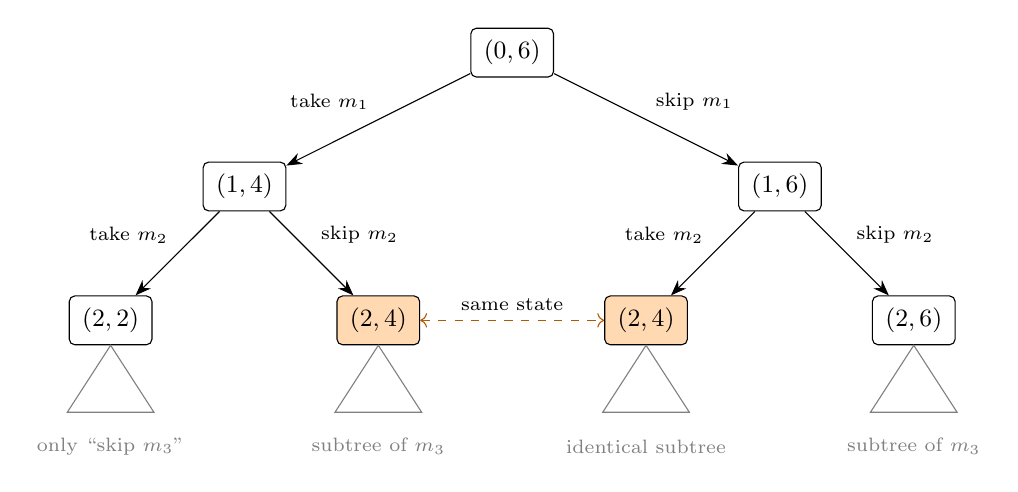
\begin{tikzpicture}[
  state/.style={draw,rounded corners=2pt,minimum width=1.05cm,minimum height=0.62cm,font=\small},
  shared/.style={fill=orange!30},
  edge/.style={-{Stealth[length=2mm]},font=\scriptsize}]
\node[state] (r) at (0,0) {$(0,6)$};
\node[state] (a) at (-3.4,-1.7) {$(1,4)$};
\node[state] (b) at (3.4,-1.7) {$(1,6)$};
\node[state] (aa) at (-5.1,-3.4) {$(2,2)$};
\node[state,shared] (ab) at (-1.7,-3.4) {$(2,4)$};
\node[state,shared] (ba) at (1.7,-3.4) {$(2,4)$};
\node[state] (bb) at (5.1,-3.4) {$(2,6)$};
\draw[edge] (r) -- node[above left] {take $m_1$} (a);
\draw[edge] (r) -- node[above right] {skip $m_1$} (b);
\draw[edge] (a) -- node[above left] {take $m_2$} (aa);
\draw[edge] (a) -- node[above right] {skip $m_2$} (ab);
\draw[edge] (b) -- node[above left] {take $m_2$} (ba);
\draw[edge] (b) -- node[above right] {skip $m_2$} (bb);
\foreach \n in {aa,ab,ba,bb}{
  \draw[gray] (\n.south) -- ++(-0.55,-0.85) -- ++(1.1,0) -- cycle;
}
\node[font=\scriptsize,gray] at (-5.1,-5.0) {only ``skip $m_3$''};
\node[font=\scriptsize,gray] at (-1.7,-5.0) {subtree of $m_3$};
\node[font=\scriptsize,gray] at (1.7,-5.0) {identical subtree};
\node[font=\scriptsize,gray] at (5.1,-5.0) {subtree of $m_3$};
\draw[<->,dashed,orange!70!black] (ab.east) -- node[above,font=\scriptsize,text=black] {same state} (ba.west);
\end{tikzpicture}
\caption{Decision tree for three modules with times $w=(2,2,3)$ and budget $T=6$. A node $(i,t)$ means that modules $1,\dots,i$ were decided and $t$ time units remain. The two shaded nodes are the same state, reached by different decisions, and their subtrees are identical: the DFS explores both, a dynamic program explores one.}\label{fig:tree}
\end{figure}

\paragraph{Logic.} The key observation is that the best score obtainable from the undecided modules depends only on the pair $(i,t)$ and not on the path that led to it. Let $F(i,t)$ be the best score using modules $i+1,\dots,n$ within $t$ time units. Then $F(n,t)=0$ and
\begin{equation}
F(i,t)=\begin{cases}
F(i+1,t) & \text{if } w_{i+1}>t,\\
\max\{F(i+1,t),\; v_{i+1}+F(i+1,t-w_{i+1})\} & \text{otherwise.}
\end{cases}
\label{eq:suffix}
\end{equation}
There are only $n(T+1)$ distinct pairs $(i,t)$ with $0\le i<n$, in contrast to the $2^n$ leaves. Caching $F$ in the recursion gives the \emph{memoized} top-down algorithm (\code{dp\_memoized}); filling a table in dependency order gives the \emph{bottom-up} algorithm (\code{dp\_table}). The table in the code uses the equivalent prefix formulation of Section~\ref{sec:design-dp}. In short, \textbf{dynamic programming is the authors' DFS with memoization}, which is why it keeps the exactness of the exhaustive search and discards its redundancy.

\subsection{The proposed technique: dynamic programming}\label{sec:design-dp}

\paragraph{Logic.} Let $D[i][t]$ be the best score obtainable from the first $i$ modules within at most $t$ time units. Then $D[0][t]=0$ for every $t$, and for $i\ge1$
\begin{equation}
D[i][t]=\begin{cases}
D[i-1][t] & \text{if } w_i>t,\\
\max\{D[i-1][t],\; D[i-1][t-w_i]+v_i\} & \text{otherwise.}
\end{cases}
\label{eq:prefix}
\end{equation}
The first case says that module $i$ does not fit and cannot be used. In the second case there are exactly two options: leave module $i$ out (the best is $D[i-1][t]$) or take it, which consumes $w_i$ units and adds $v_i$ points, leaving $t-w_i$ units for the first $i-1$ modules. The recurrence refers to row $i-1$, never to row $i$, so each module is used at most once: this is what makes the problem 0/1 instead of unbounded.

\paragraph{Execution steps.}
\begin{enumerate}[leftmargin=1.6em,itemsep=1pt]
\item \emph{Initialization:} fill row $0$ with zeros.
\item \emph{Fill:} for $i=1,\dots,n$ and $t=0,\dots,T$, apply Equation~\eqref{eq:prefix}.
\item \emph{Read the optimum:} $D[n][T]$ is the maximum score.
\item \emph{Reconstruct:} start at $(i,t)=(n,T)$. If $D[i][t]\neq D[i-1][t]$, module $i$ was taken: record it and set $t\leftarrow t-w_i$. In either case set $i\leftarrow i-1$.
\end{enumerate}

\paragraph{Useful properties.} Because $D[i][t]$ is defined for \emph{at most} $t$ units, the last row $D[n][\cdot]$ contains the optimum for \emph{every} budget up to $T$, and the reconstruction works for any of them. This answers for free the natural question of a learner: ``what if I had only 8 hours?''. The table needs $(n+1)(T+1)$ cells; since a row depends only on the previous one, a single vector of $T+1$ cells suffices if $t$ is scanned in decreasing order (otherwise the already-updated value would be reused and a module could be taken several times) at the price of losing the reconstruction (\code{dp\_vector}).

\subsection{The comparison technique: greedy strategy}\label{sec:design-greedy}

\paragraph{Motivation.} The fractional knapsack is solved exactly by taking modules in decreasing order of $v_i/w_i$ (Section~\ref{sec:knapsack}). It is natural to try the same rule when modules are indivisible: it is simple and extremely fast.

\paragraph{Logic and steps.} (1) Sort the modules by decreasing ratio; (2) scan them in this order and take every module that still fits. The sort is a merge sort, an instance of divide and conquer: \emph{divide} the list into two halves, \emph{conquer} by sorting each half recursively, \emph{combine} by merging the two sorted halves. Ratios are compared by cross-multiplication ($v_iw_j > v_jw_i$), avoiding divisions and floating-point issues, and the merge is stable.

\paragraph{Why it can fail.} Because modules cannot be split, a short module with a high ratio can consume time that prevents a better combination. On the test instance the greedy takes modules 1, 2, 4 and 6 (9~h, score 77) while the optimum is modules 2 and 3 (10~h, score 91). The variant \code{greedy\_with\_best\_item} returns the better of the greedy solution and the best single module, which repairs the worst pathologies (Proposition~\ref{prop:greedy-half}).

\subsection{Additional algorithms}\label{sec:design-extra}

\paragraph{Branch and Bound.} \emph{Motivation:} the DFS explores subtrees that clearly cannot win. \emph{Logic:} sort the modules by ratio; at each node compute an upper bound by filling the remaining room with whole modules in ratio order and a fraction of the first one that does not fit (floored, because scores are integers); if the bound does not exceed the best known score, discard the subtree. \emph{Steps:} as in the DFS, plus the bound test before expanding a node.

\paragraph{Meet-in-the-Middle.} \emph{Motivation:} reduce $2^n$ to about $2^{n/2}$ without depending on $T$. \emph{Logic:} split the modules into halves $A$ and $B$; enumerate the feasible subsets of each half sorted by time; for each subset of $A$, the best partner in $B$ is the best subset whose time is at most $T$ minus the time of the $A$-subset. \emph{Steps:} (1) generate each half's subsets by merging a list with its shifted copy, which keeps it sorted by time; (2) precompute for $B$ the best score among the subsets up to each position; (3) sweep $A$ in increasing time while a pointer in $B$ moves monotonically backwards.

\paragraph{FPTAS.} \emph{Motivation:} obtain a guarantee that does not depend on $T$. \emph{Logic:} scale the scores to $v'_i=\lfloor v_i/K\rfloor$ with $K=\varepsilon v_{\max}/n$, which makes the sum of scaled scores at most $n^2/\varepsilon$, and solve the scaled instance exactly with a DP over the \emph{profit}: for each scaled score, the minimum time needed to reach it. \emph{Steps:} fill the profit table, pick the largest scaled score reachable within $T$, reconstruct the modules and sum their \emph{original} scores.

\subsection{The authors' technique on the prerequisite graph}

The extension \code{graph\_dfs.py} implements the strategy of the article on a graph of modules with prerequisites: starting from a source module, it enumerates every simple path whose accumulated time fits the budget, records the path with the highest score and uses backtracking to leave each path. On a complete DAG (an edge from $i$ to every $j>i$) every subset of the other $n-1$ nodes, taken in order, is a path, so there are $2^{n-1}$ paths; Section~\ref{sec:exp-graph} confirms this count.

\section{Implementation}\label{sec:implementation}

\subsection{Environment and architecture}

The prototype is written in Python (the reported experiments ran on Python 3.12; version 3.10 or newer is required) using only the standard library; the matplotlib library is used exclusively to draw the plots of Section~\ref{sec:experiments} and does not take part in any algorithm. Even the sorting routine is hand-written. The code runs on Linux with a single command (Appendix~\ref{app:run}). Its organization follows the two files requested by the assignment: the \emph{Algorithm} files and the \emph{Experiment} file.

\begin{table}[h]
\centering
\caption{Organization of the source code.}\label{tab:files}
\small
\begin{tabularx}{\linewidth}{@{}l X@{}}
\toprule
File & Content\\
\midrule
\code{algorithms/model.py} & \code{LearningModule} (name, time, score), \code{Result} (algorithm, value, indices, operations), instance validation and evaluation of a selection\\
\code{algorithms/sorting.py} & Stable hand-written merge sort; \code{sort\_by\_ratio} compares ratios by cross-multiplication\\
\code{algorithms/dfs.py} & \code{exhaustive\_dfs}: the authors' strategy (decision tree, pruning, backtracking)\\
\code{algorithms/graph\_dfs.py} & \code{dfs\_paths}, \code{complete\_dag}: DFS over the prerequisite graph\\
\code{algorithms/dp.py} & \code{dp\_table}, \code{dp\_vector}, \code{dp\_memoized}: the proposed dynamic programming\\
\code{algorithms/greedy.py} & \code{greedy}, \code{greedy\_with\_best\_item}: comparison algorithm and its variant with a guarantee\\
\code{algorithms/branch\_and\_bound.py} & \code{branch\_and\_bound}\\
\code{algorithms/meet\_in\_the\_middle.py} & \code{meet\_in\_the\_middle}\\
\code{algorithms/fptas.py} & \code{fptas}\\
\code{instances.py} & \code{generate\_instance}: the three instance families, reproducible by seed\\
\code{experiment.py} & \textbf{Experiment file}: the test instance and nine blocks of experiments (command-line selectable)\\
\bottomrule
\end{tabularx}
\end{table}

Every algorithm returns the same \code{Result} type, which makes comparisons and tests uniform and avoids duplicated code. The field \code{operations} is a deterministic counter of elementary steps whose meaning is fixed per algorithm (Table~\ref{tab:ops}).

\begin{table}[h]
\centering
\caption{What each operation counter counts.}\label{tab:ops}
\small
\begin{tabularx}{\linewidth}{@{}l X@{}}
\toprule
Algorithm & Counted operations\\
\midrule
\code{exhaustive\_dfs} & nodes of the decision tree visited\\
\code{dp\_table} & table cells computed, exactly $n(T+1)$\\
\code{dp\_vector} & iterations of the inner loop\\
\code{dp\_memoized} & distinct states $(i,t)$ computed ($\le n(T+1)$)\\
\code{greedy} & comparisons of the merge sort plus one step per module scanned\\
\code{greedy\_with\_best\_item} & as \code{greedy}, plus $n$ steps to find the best single module\\
\code{branch\_and\_bound} & nodes visited, plus steps spent computing upper bounds, plus sort comparisons\\
\code{meet\_in\_the\_middle} & subset entries generated, merge comparisons and pointer steps\\
\code{fptas} & cells of the profit table\\
\bottomrule
\end{tabularx}
\end{table}

\subsection{Pseudocode}

\SetKwProg{Proc}{Procedure}{}{}
\newcommand{\FExplore}{\mathrm{Explore}}
\newcommand{\FBest}{\mathrm{Best}}
\newcommand{\FUB}{\mathrm{UpperBound}}
\newcommand{\FSubsets}{\mathrm{Subsets}}

\begin{algorithm}[htbp]
\caption{Exhaustive DFS with pruning and backtracking (\code{exhaustive\_dfs})}\label{alg:dfs}
\KwIn{modules $(w_i,v_i)$, $i=1..n$; budget $T$}
\KwOut{best score $best$ and the selected modules $bestSet$}
$best \leftarrow 0$;\quad $chosen \leftarrow [\,]$;\quad $bestSet \leftarrow [\,]$\;
\Proc{$\FExplore(i,u,s)$}{
  \If{$s>best$}{$best\leftarrow s$;\quad $bestSet\leftarrow \mathrm{copy}(chosen)$\;}
  \lIf{$i=n$}{\Return}
  \If{$u+w_{i+1}\le T$}{
    append $i+1$ to $chosen$\;
    $\FExplore(i+1,\ u+w_{i+1},\ s+v_{i+1})$\;
    remove $i+1$ from $chosen$ \Comment*{backtracking}
  }
  $\FExplore(i+1,\ u,\ s)$\;
}
$\FExplore(0,0,0)$\;
\Return $best,\ bestSet$\;
\end{algorithm}

\begin{algorithm}[htbp]
\caption{Dynamic programming: table and reconstruction (\code{dp\_table})}\label{alg:dp}
\KwIn{modules $(w_i,v_i)$, $i=1..n$; budget $T$}
\KwOut{optimal score $D[n][T]$ and the selected modules $chosen$}
\lFor{$t\leftarrow 0$ \KwTo $T$}{$D[0][t]\leftarrow 0$}
\For{$i\leftarrow 1$ \KwTo $n$}{
  \For{$t\leftarrow 0$ \KwTo $T$}{
    $D[i][t]\leftarrow D[i-1][t]$ \Comment*{do not take module $i$}
    \If{$w_i\le t$ \textbf{and} $D[i-1][t-w_i]+v_i>D[i][t]$}{
      $D[i][t]\leftarrow D[i-1][t-w_i]+v_i$ \Comment*{take module $i$}
    }
  }
}
$t\leftarrow T$;\quad $chosen\leftarrow[\,]$\;
\For{$i\leftarrow n$ \textbf{down to} $1$}{
  \If{$D[i][t]\neq D[i-1][t]$}{prepend $i$ to $chosen$;\quad $t\leftarrow t-w_i$\;}
}
\Return $D[n][T],\ chosen$\;
\end{algorithm}

\begin{algorithm}[htbp]
\caption{Dynamic programming with memoization (\code{dp\_memoized})}\label{alg:memo}
\KwIn{modules $(w_i,v_i)$, $i=1..n$; budget $T$}
\KwOut{optimal score $\FBest(0,T)$}
$memo\leftarrow$ empty map\;
\Proc{$\FBest(i,t)$}{
  \lIf{$i=n$}{\Return $0$}
  \lIf{$(i,t)\in memo$}{\Return $memo[(i,t)]$}
  $r\leftarrow\FBest(i+1,t)$\;
  \lIf{$w_{i+1}\le t$}{$r\leftarrow\max\{r,\ v_{i+1}+\FBest(i+1,t-w_{i+1})\}$}
  $memo[(i,t)]\leftarrow r$;\quad \Return $r$\;
}
\end{algorithm}

\begin{algorithm}[htbp]
\caption{Greedy by ratio, with the best-single-module variant (\code{greedy}, \code{greedy\_with\_best\_item})}\label{alg:greedy}
\KwIn{modules $(w_i,v_i)$, $i=1..n$; budget $T$}
\KwOut{score $G$ (greedy) and score $\max\{G,M\}$ (variant)}
$order\leftarrow$ \textsc{MergeSort}(modules, $i$ before $j$ iff $v_iw_j>v_jw_i$)\;
$u\leftarrow 0$;\quad $G\leftarrow 0$\;
\ForEach{$i$ \textbf{in} $order$}{
  \If{$u+w_i\le T$}{$u\leftarrow u+w_i$;\quad $G\leftarrow G+v_i$\;}
}
$M\leftarrow\max\{v_i : w_i\le T\}$ \Comment*{variant only}
\Return $G$ \textbf{and} $\max\{G,M\}$\;
\end{algorithm}

\begin{algorithm}[htbp]
\caption{Branch and Bound with the fractional bound (\code{branch\_and\_bound})}\label{alg:bb}
\KwIn{modules $(w_i,v_i)$, $i=1..n$; budget $T$}
\KwOut{optimal score $best$}
$o\leftarrow$ modules sorted by decreasing $v/w$;\quad $best\leftarrow0$;\quad $chosen\leftarrow[\,]$\;
\Proc{$\FUB(k,u,s)$}{
  $room\leftarrow T-u$;\quad $ub\leftarrow s$\;
  \For{$j\leftarrow k+1$ \KwTo $n$}{
    \lIf{$w_{o_j}\le room$}{$room\leftarrow room-w_{o_j}$;\quad $ub\leftarrow ub+v_{o_j}$}
    \lElse{\Return $ub+\lfloor room\cdot v_{o_j}/w_{o_j}\rfloor$}
  }
  \Return $ub$\;
}
\Proc{$\FExplore(k,u,s)$}{
  $best\leftarrow\max\{best,s\}$\;
  \lIf{$k=n$ \textbf{or} $\FUB(k,u,s)\le best$}{\Return}
  \If{$u+w_{o_{k+1}}\le T$}{take $o_{k+1}$, $\FExplore(k+1,\ u+w_{o_{k+1}},\ s+v_{o_{k+1}})$, undo\;}
  $\FExplore(k+1,\ u,\ s)$\;
}
$\FExplore(0,0,0)$\;
\end{algorithm}

\begin{algorithm}[htbp]
\caption{Meet-in-the-Middle (\code{meet\_in\_the\_middle})}\label{alg:mitm}
\KwIn{modules $(w_i,v_i)$, $i=1..n$; budget $T$}
\KwOut{optimal score $best$}
split the modules into halves $A$ (first $\lfloor n/2\rfloor$) and $B$ (the rest)\;
\Proc{$\FSubsets(H)$}{
  $L\leftarrow[(0,0)]$ \Comment*{pairs (time, score), sorted by time}
  \ForEach{module $j$ \textbf{in} $H$}{
    $L'\leftarrow[(t+w_j,\ s+v_j) : (t,s)\in L,\ t+w_j\le T]$\;
    $L\leftarrow\textsc{Merge}(L,L')$ by time \Comment*{stays sorted}
  }
  \Return $L$\;
}
$L_A\leftarrow\FSubsets(A)$;\quad $L_B\leftarrow\FSubsets(B)$\;
$bestB[j]\leftarrow$ largest score among $L_B[0..j]$;\quad $p\leftarrow |L_B|-1$;\quad $best\leftarrow0$\;
\ForEach{$(t,s)$ \textbf{in} $L_A$ \textnormal{(increasing $t$)}}{
  \While{time of $L_B[p]$ $+\ t>T$}{$p\leftarrow p-1$\;}
  $best\leftarrow\max\{best,\ s+bestB[p]\}$\;
}
\Return $best$\;
\end{algorithm}

\begin{algorithm}[htbp]
\caption{FPTAS by profit scaling (\code{fptas})}\label{alg:fptas}
\KwIn{modules $(w_i,v_i)$ with $w_i\le T$; budget $T$; accuracy $\varepsilon$}
\KwOut{a selection with score $\ge(1-\varepsilon)\,\OPT$}
$K\leftarrow\varepsilon\cdot v_{\max}/n$;\quad $v'_i\leftarrow\lfloor v_i/K\rfloor$;\quad $S\leftarrow\sum_i v'_i$\;
$W[0][0]\leftarrow0$;\quad $W[0][s]\leftarrow\infty$ for $s>0$ \Comment*{$W[k][s]$: least time to reach scaled score $s$}
\For{$k\leftarrow1$ \KwTo $n$}{
  \For{$s\leftarrow0$ \KwTo $S$}{
    $W[k][s]\leftarrow W[k-1][s]$\;
    \If{$s\ge v'_k$ \textbf{and} $W[k-1][s-v'_k]+w_k\le T$ \textbf{and} $W[k-1][s-v'_k]+w_k<W[k][s]$}{
      $W[k][s]\leftarrow W[k-1][s-v'_k]+w_k$\;
    }
  }
}
$s^*\leftarrow\max\{s : W[n][s]\le T\}$;\quad reconstruct the modules as in Algorithm~\ref{alg:dp}\;
\Return the selected modules and the sum of their \emph{original} scores\;
\end{algorithm}

\FloatBarrier
\subsection{Test instance}\label{sec:testinstance}

The test instance models a learner with a budget of $T=10$ hours choosing among six modules (Table~\ref{tab:instance}). It is defined in \code{test\_instance()} and executed by the block \code{demo} of \code{experiment.py}.

\begin{table}[h]
\centering
\caption{Test instance ($T=10$ h).}\label{tab:instance}
\small
\begin{tabular}{@{}c l r r r@{}}
\toprule
$i$ & Module & Hours $w_i$ & Score $v_i$ & Ratio $v_i/w_i$\\
\midrule
1 & Programming Logic & 1 & 10 & 10.0\\
2 & Python Basics & 5 & 46 & 9.2\\
3 & Data Structures & 5 & 45 & 9.0\\
4 & Databases & 2 & 15 & 7.5\\
5 & Networking & 3 & 20 & 6.7\\
6 & Git & 1 & 6 & 6.0\\
\bottomrule
\end{tabular}
\end{table}

Table~\ref{tab:dptable} shows the table $D[i][t]$ produced by the code. The shaded cells are visited by the reconstruction, which starts at $D[6][10]=91$. At $i=6$, $5$ and $4$ the value does not change when module $i$ is removed ($D[i][10]=D[i-1][10]$), so Git, Networking and Databases are not taken. At $i=3$, $D[3][10]=91\neq D[2][10]=56$: Data Structures is taken and the remaining time is $10-5=5$. At $i=2$, $D[2][5]=46\neq D[1][5]=10$: Python Basics is taken and the remaining time is $0$. The optimal selection is therefore modules 2 and 3, using 10 hours and scoring 91.

\begin{table}[h]
\centering
\caption{Dynamic-programming table for the test instance. Rows: modules considered; columns: available time $t$. Shaded: cells visited by the reconstruction; bold: modules taken.}\label{tab:dptable}
\small
\begin{tabular}{c|rrrrrrrrrrr}
\toprule
$i \backslash t$ & 0 & 1 & 2 & 3 & 4 & 5 & 6 & 7 & 8 & 9 & 10 \\
\midrule
0 & \cellcolor{green!25}0 & 0 & 0 & 0 & 0 & 0 & 0 & 0 & 0 & 0 & 0 \\
1 & \cellcolor{green!25}0 & 10 & 10 & 10 & 10 & 10 & 10 & 10 & 10 & 10 & 10 \\
2 & 0 & 10 & 10 & 10 & 10 & \cellcolor{green!25}\textbf{46} & 56 & 56 & 56 & 56 & 56 \\
3 & 0 & 10 & 10 & 10 & 10 & 46 & 56 & 56 & 56 & 56 & \cellcolor{green!25}\textbf{91} \\
4 & 0 & 10 & 15 & 25 & 25 & 46 & 56 & 61 & 71 & 71 & \cellcolor{green!25}91 \\
5 & 0 & 10 & 15 & 25 & 30 & 46 & 56 & 61 & 71 & 76 & \cellcolor{green!25}91 \\
6 & 0 & 10 & 16 & 25 & 31 & 46 & 56 & 62 & 71 & 77 & \cellcolor{green!25}91 \\
\bottomrule
\end{tabular}

\end{table}

The greedy algorithm sorts the modules by ratio (1, 2, 3, 4, 5, 6), takes modules 1, 2, 4 and 6 (9 hours, score 77), and skips 3 and 5 because they no longer fit. It ends 15.4\% below the optimum because module 1, with the highest ratio, uses an hour that prevents the ideal pair from fitting. Table~\ref{tab:instance-results} lists the result of every algorithm; all exact algorithms return 91.

\begin{table}[h]
\centering
\caption{Results on the test instance (output of \code{python experiment.py --only demo}).}\label{tab:instance-results}
\small
\begin{tabular}{@{}l r l r r@{}}
\toprule
Algorithm & Score & Selected modules & Hours used & Operations\\
\midrule
Exhaustive DFS & 91 & 2, 3 & 10 & 93\\
DP (table) & 91 & 2, 3 & 10 & 66 ($=6\times11$)\\
DP (vector) & 91 & --- (value only) & --- & 49\\
DP (memoized) & 91 & 2, 3 & 10 & 32 states\\
Branch and Bound & 91 & 2, 3 & 10 & 70\\
Meet-in-the-Middle & 91 & 2, 3 & 10 & 46\\
FPTAS ($\varepsilon=0.1$) & 91 & 2, 3 & 10 & 1,098\\
Greedy & 77 & 1, 2, 4, 6 & 9 & 13\\
Greedy + best item & 77 & 1, 2, 4, 6 & 9 & 19\\
\bottomrule
\end{tabular}
\end{table}

The memoized DP visits 32 states, well below the 66 cells of the table and the 93 nodes of the DFS, which illustrates the link between the three algorithms discussed in Section~\ref{sec:design-bridge}. An \emph{adversarial instance} shows that the greedy can be arbitrarily bad: with $T=1000$, a short module with 1 hour and 2 points (ratio 2.0) and a long module with 1000 hours and 1000 points (ratio 1.0). The greedy takes the short module and obtains 2 (a gap of 99.8\%), after which the long module no longer fits; the variant with the best single module, the DP and all exact algorithms obtain 1000.

\subsection{Decisions and missing specifications}\label{sec:decisions}

The assignment asks for the decisions made and for any detail missing from its description. Ours were:

\begin{enumerate}[leftmargin=1.6em,itemsep=2pt]
\item \textbf{Relaxation without prerequisites.} The article works on a course graph; we treat modules as independent (0/1 knapsack). The version with precedence (Section~\ref{sec:background}) is left as future work. The prerequisite-graph DFS is provided separately in \code{graph\_dfs.py}.
\item \textbf{Time and score are inputs.} We do not reimplement how the article estimates module time and score; we take them as given integers.
\item \textbf{Integer time unit.} Times are positive integers (minutes or blocks of 15~minutes). This is required by the DP table and is the origin of its pseudo-polynomial nature.
\item \textbf{Details a DFS implementation must fix.} State restoration is explicit (the \texttt{pop} after the recursive call); the best selection is recorded at every node; ties keep the first optimum found (strict comparison); modules are visited in input order (only Branch and Bound uses ratio order).
\item \textbf{Own merge sort.} We implement a stable merge sort instead of the built-in \code{sorted}. This keeps the greedy at $\Theta(n\log n)$ in every case (Python's Timsort runs in $\mathcal{O}(n)$ on already sorted input, which would blur the best-case analysis) and respects the rule against relying on library implementations.
\item \textbf{Exact arithmetic.} Ratios are compared by cross-multiplication and scores are integers, so there are no floating-point ties in the exact algorithms; only the FPTAS uses a floating-point scaling constant.
\item \textbf{Counters and timing.} Conclusions rely on operation counters (Table~\ref{tab:ops}); wall-clock time is the median of three executions (one execution when the DFS exceeds 18 modules).
\item \textbf{DFS size limit.} The DFS is run only up to $n=22$ in the timing experiments, because its cost doubles with each additional module.
\item \textbf{Instance families.} The strongly correlated family uses the constant $R/2$ instead of the $R/10$ usual in the literature, to make the effect clearly visible with small ranges; this is a deviation we state explicitly (Section~\ref{sec:method}).
\end{enumerate}

\section{Complexity Analysis}\label{sec:complexity}

This section addresses assignment item 1.1.2. For each algorithm we prove its correctness (when the analysis depends on it) and derive its best-case, worst-case and space complexity; the average case is measured empirically in Section~\ref{sec:experiments}, because it depends on the distribution of the instances.

\subsection{Conventions}

An \emph{elementary operation} is the unit counted by the corresponding counter in Table~\ref{tab:ops}. We use $n$ for the number of modules, $T$ for the budget and $w_i\ge1$ for integer times. Inputs in which some or all modules do not fit are valid and are accepted by the code (the best case of the DFS occurs on one of them). When we reason about solutions (approximation guarantees), we assume without loss of generality that $w_i\le T$ for every $i$, since a module that does not fit alone belongs to no feasible solution and removing it changes neither $\OPT$ nor the value returned by the algorithms.

\subsection{Exhaustive DFS}

\begin{theorem}[Correctness of the DFS]\label{thm:dfs-correct}
Algorithm~\ref{alg:dfs} returns the maximum score over all feasible selections.
\end{theorem}
\begin{proof}
Every node $(i,u,s)$ visited corresponds to the feasible selection $chosen\subseteq\{1,\dots,i\}$ with time $u\le T$ and score $s$, because a module is appended only if $u+w_{i+1}\le T$ and is removed on backtracking. Conversely, every feasible selection $S$ is visited: following the decisions of $S$ from the root, every ``take'' decision is allowed because the accumulated time never exceeds $w(S)\le T$. The algorithm records the best score over all visited nodes, hence it returns $\max\{v(S): w(S)\le T\}$.
\end{proof}

\begin{proposition}[Number of nodes]\label{prop:dfs-nodes}
Let $N$ be the number of nodes visited by Algorithm~\ref{alg:dfs}. Then $n+1\le N\le 2^{n+1}-1$. Moreover, $N=2^{n+1}-1$ if and only if $\sum_i w_i\le T$, and $N=n+1$ if and only if $w_i>T$ for all $i$.
\end{proposition}
\begin{proof}
The ``skip'' branch is always available, so the path that skips every module exists and has $n+1$ nodes: $N\ge n+1$. Each internal node has at most two children and the depth is $n$, so the tree has at most $\sum_{k=0}^{n}2^k=2^{n+1}-1$ nodes. Equality holds exactly when every ``take'' branch is feasible, in which case $N$ satisfies $N(i)=1+2N(i+1)$ with $N(n)=1$, i.e.\ $N=2^{n+1}-1$. This happens when the path that takes all modules is feasible, which is equivalent to $\sum_i w_i\le T$ (all other paths use less time). The lower bound is attained when no ``take'' branch is ever feasible; as the all-skip path keeps the used time at zero, this means $w_i>T$ for all $i$.
\end{proof}

\paragraph{Best, worst and space.} The running time is $\Theta(N)$ (up to the cost of copying the incumbent solution, $\bigO(n)$ each time it improves; this is the usual convention for tree searches and the factor can be removed by recording the incumbent differently). Hence the best case is $\Theta(n)$ and the worst case is $\Theta(2^n)$. The recursion depth is $n+1$ and the list \emph{chosen} has at most $n$ elements, so the space is $\Theta(n)$. The average case depends on how generous the budget is; it is measured in Section~\ref{sec:exp-dfs}.

\subsection{Dynamic programming}

\begin{lemma}[Recurrence]\label{lem:rec}
For all $0\le i\le n$ and $0\le t\le T$, the value $D[i][t]$ computed by Equation~\eqref{eq:prefix} equals $\max\{v(S): S\subseteq\{1,\dots,i\},\ w(S)\le t\}$.
\end{lemma}
\begin{proof}
By induction on $i$. For $i=0$ the only subset is $\emptyset$, whose score is 0, as in $D[0][t]=0$. Let $i\ge1$ and let $S$ be an optimal subset for $(i,t)$. If $w_i>t$, module $i$ cannot belong to $S$, so $S$ is a feasible subset of $\{1,\dots,i-1\}$ and, by induction, its value is at most $D[i-1][t]$, which is achievable; this is the first case of the recurrence. If $w_i\le t$, either $i\notin S$, and then $v(S)\le D[i-1][t]$; or $i\in S$, and then $S\setminus\{i\}$ is a subset of $\{1,\dots,i-1\}$ with time at most $t-w_i$, so $v(S)\le v_i+D[i-1][t-w_i]$. Both values are achievable by the induction hypothesis, hence the optimum is their maximum, as in the second case.
\end{proof}

\begin{lemma}[Reconstruction]\label{lem:reconstruction}
The backward walk of Algorithm~\ref{alg:dp} returns a feasible selection with score $D[n][T]$.
\end{lemma}
\begin{proof}
Invariant: at the start of the iteration for $i$ with current time $t$, the selected modules so far plus the optimal value of $(i,t)$ add up to $D[n][T]$. If $D[i][t]\neq D[i-1][t]$, then by the recurrence $D[i][t]>D[i-1][t]$ and $D[i][t]=D[i-1][t-w_i]+v_i$: module $i$ is taken, the invariant holds for $(i-1,t-w_i)$, and the time remains non-negative because $w_i\le t$. If $D[i][t]=D[i-1][t]$, the invariant holds for $(i-1,t)$ without taking $i$. At $i=0$ the remaining value is 0.
\end{proof}

\begin{theorem}[Complexity of the DP]\label{thm:dp}
Algorithm~\ref{alg:dp} computes exactly $n(T+1)$ cells, each in constant time. Its running time is $\Theta(nT)$ in the best, worst and average cases, and the reconstruction adds $\Theta(n)$. The space is $\Theta(nT)$ for the table and $\Theta(T)$ for the vector version (which runs at most $n(T+1)$ inner iterations).
\end{theorem}
\begin{proof}
The loops have fixed bounds $n$ and $T+1$ that do not depend on the values of $w_i$ and $v_i$, and the body does a constant number of comparisons and additions. Hence the count is $n(T+1)$ on every input. The table has $(n+1)(T+1)$ cells. In the vector version, row $i$ is computed from row $i-1$ in place by scanning $t$ from $T$ down to $w_i$; the decreasing order guarantees that $d[t-w_i]$ still holds the value of row $i-1$.
\end{proof}

\begin{proposition}[Pseudo-polynomial time]\label{prop:pseudo}
The running time $\Theta(nT)$ is polynomial in the numeric value of $T$ but exponential in the length of its binary encoding.
\end{proposition}
\begin{proof}
Writing $T$ takes $k=\lceil\log_2(T+1)\rceil$ bits, so $T\ge 2^{k-1}$ and the running time is $\Omega(n2^{k-1})$, exponential in $k$. It is polynomial only if $T$ is bounded by a polynomial in $n$ (or if numbers are encoded in unary). This does not contradict the NP-hardness of the problem, which would be contradicted only by an algorithm polynomial in the \emph{bit length} of the input.
\end{proof}

\paragraph{Memoized version.} The reachable states $(i,t)$ satisfy $0\le i<n$ and $0\le t\le T$, so at most $n(T+1)$ states are computed, each in constant time besides the recursive calls: $\bigO(nT)$ in the worst case. If no module fits, only the states $(0,T),\dots,(n-1,T)$ are visited: the best case is $\Theta(n)$. The space is $\bigO(nT)$ for the cache and $\Theta(n)$ for the recursion.

\subsection{Greedy strategy}

\begin{proposition}[Running time]\label{prop:greedy-time}
The greedy algorithm runs in $\Theta(n\log n)$ in the best, worst and average cases, using $\Theta(n)$ space.
\end{proposition}
\begin{proof}
Merging two sorted lists of sizes $a\le b$ takes between $a$ and $a+b-1$ comparisons. For the balanced halves of merge sort, the cost $m(n)$ of the merge step satisfies $\lfloor n/2\rfloor\le m(n)\le n-1$, so the number of comparisons $C(n)=C(\lfloor n/2\rfloor)+C(\lceil n/2\rceil)+m(n)$ is $\Theta(n\log n)$ by the master theorem, regardless of the order of the input. The scan that follows takes $\Theta(n)$ steps. The lists and the output use $\Theta(n)$ space.
\end{proof}

\begin{proposition}[The greedy has no constant approximation ratio]\label{prop:greedy-unbounded}
For every $T\ge3$ there is an instance on which the greedy obtains value $2$ while $\OPT=T$; the ratio $2/T$ tends to $0$.
\end{proposition}
\begin{proof}
Take two modules $(w_1,v_1)=(1,2)$ and $(w_2,v_2)=(T,T)$. The ratios are $2$ and $1$, so the greedy takes module 1 first; then $1+T>T$ and module 2 does not fit. The greedy value is $2$, while module 2 alone is feasible and has value $T>2$.
\end{proof}

\begin{proposition}[Greedy with the best single module]\label{prop:greedy-half}
Let $G$ be the value of the greedy solution and $M=\max\{v_i: w_i\le T\}$. Then $\max\{G,M\}\ge\OPT/2$.
\end{proposition}
\begin{proof}
Order the modules by decreasing ratio. If all modules fit together, $G=\OPT$. Otherwise let $k$ be the first module in this order that does not fit when the greedy reaches it; the greedy has taken all modules $1,\dots,k-1$, so $G\ge P:=\sum_{i<k}v_i$. By Dantzig's fractional relaxation \cite{dantzig1957}, $\OPT\le P+\frac{r}{w_k}v_k\le P+v_k$, where $r<w_k$ is the room left after the first $k-1$ modules. Since $w_k\le T$, we have $v_k\le M$, so $\OPT\le G+M\le 2\max\{G,M\}$.
\end{proof}

\subsection{Branch and Bound}

\begin{lemma}[Validity of the bound]\label{lem:bound}
For a node at position $k$ with used time $u$ and score $s$, the quantity $s+\lfloor\mathrm{fill}\rfloor$ computed by \textsc{UpperBound} is at least the best score of any selection that extends the node.
\end{lemma}
\begin{proof}
The undecided modules, taken in decreasing ratio, are filled until the first one that does not fit, of which a fraction is taken: this is the optimal solution of the fractional relaxation of the remaining problem \cite{dantzig1957}. Any integral extension is feasible for the relaxation, so its value is at most the relaxation value; since scores are integers, it is also at most the floor of that value.
\end{proof}

\paragraph{Correctness and complexity.} Pruning a node whose bound does not exceed the incumbent discards only extensions that cannot improve it (Lemma~\ref{lem:bound}), so Branch and Bound returns the optimum, by the same argument as Theorem~\ref{thm:dfs-correct}. It visits at most $2^{n+1}-1$ nodes and spends $\bigO(n)$ steps on the bound of each, so the worst case is $\bigO(n2^n)$. The sort costs $\Theta(n\log n)$, which is also the best case (for example, when no module fits). The behavior in between depends on how tight the bound is, which in turn depends on the instance family (Section~\ref{sec:exp-families}). The space is $\Theta(n)$.

\subsection{Meet-in-the-Middle}

\begin{theorem}[Meet-in-the-Middle]\label{thm:mitm}
The algorithm is exact and runs in $\bigO(2^{\lceil n/2\rceil})$ time and space, regardless of $T$. This bound is tight (worst case $\Theta(2^{n/2})$) when $\sum_i w_i\le T$, and the best case is $\Theta(n)$ when no module fits.
\end{theorem}
\begin{proof}
After processing $k$ modules, each list holds at most $2^k$ subsets, and the merge of a list with its shifted copy costs $\bigO(2^k)$. Summing over the $h=\lceil n/2\rceil$ modules of the larger half gives $\sum_{k<h}\bigO(2^k)=\bigO(2^h)$; the sweep of the second phase is linear in $|L_A|+|L_B|$. Correctness: as $t$ (the time of the subset of $A$) grows, the room $T-t$ shrinks, so the pointer in $L_B$ only moves backwards; $bestB[p]$ is the best score among the subsets of $B$ with time at most the time at position $p$, hence the sweep evaluates $\max_{a}\,\bigl(v_a+\mathrm{best}_B(T-t_a)\bigr)$ over all subsets $a$ of $A$, which equals $\OPT$. If $\sum_iw_i\le T$ nothing is pruned and both lists are complete. If no module fits, both lists remain $[(0,0)]$ and the merges are trivial: $\Theta(n)$.
\end{proof}

\subsection{FPTAS}

\begin{theorem}[FPTAS guarantee and cost]\label{thm:fptas}
For $\varepsilon\in(0,1)$, Algorithm~\ref{alg:fptas} returns a feasible selection with value at least $(1-\varepsilon)\OPT$ in $\bigO(n^3/\varepsilon)$ time and space.
\end{theorem}
\begin{proof}
Let $S^*$ be an optimal selection and $S'$ the selection returned, optimal for the scaled scores $v'_i=\lfloor v_i/K\rfloor$ (the profit DP is exact). Since $K v'_i\le v_i<Kv'_i+K$,
\[
v(S')\ \ge\ K\,v'(S')\ \ge\ K\,v'(S^*)\ >\ \sum_{i\in S^*}(v_i-K)\ \ge\ \OPT-nK\ =\ \OPT-\varepsilon v_{\max}\ \ge\ (1-\varepsilon)\OPT,
\]
where the last step uses $v_{\max}\le\OPT$ (the module with the largest score fits alone). The scaled scores satisfy $v'_i\le v_{\max}/K=n/\varepsilon$, so $S=\sum_iv'_i\le n^2/\varepsilon$ and the table has $(n+1)(S+1)=\bigO(n^3/\varepsilon)$ cells, each computed in constant time.
\end{proof}

\subsection{Summary}

\begin{table}[h]
\centering
\caption{Complexity summary. Averages marked ``measured'' are reported in Section~\ref{sec:experiments}.}\label{tab:complexity}
\small
\begin{tabularx}{\linewidth}{@{}l l l X l@{}}
\toprule
Algorithm & Best case & Worst case & Average case & Space\\
\midrule
Exhaustive DFS & $\Theta(n)$ & $\Theta(2^n)$ & measured (data dependent) & $\Theta(n)$\\
DP (table) & $\Theta(nT)$ & $\Theta(nT)$ & $\Theta(nT)$ & $\Theta(nT)$\\
DP (vector) & $\Theta(nT)$ & $\Theta(nT)$ & $\Theta(nT)$ & $\Theta(T)$\\
DP (memoized) & $\Theta(n)$ states & $\bigO(nT)$ states & measured (reachable states) & $\bigO(nT)$\\
Greedy & $\Theta(n\log n)$ & $\Theta(n\log n)$ & $\Theta(n\log n)$ & $\Theta(n)$\\
Greedy + best item & $\Theta(n\log n)$ & $\Theta(n\log n)$ & $\Theta(n\log n)$ & $\Theta(n)$\\
Branch and Bound & $\Theta(n\log n)$ & $\bigO(n2^n)$ & measured (instance dependent) & $\Theta(n)$\\
Meet-in-the-Middle & $\Theta(n)$ & $\Theta(2^{n/2})$ & measured (depends on $T$) & $\bigO(2^{n/2})$\\
FPTAS & $\Theta(nS)$ & $\bigO(n^3/\varepsilon)$ & $\Theta(nS)$ with $S\le n^2/\varepsilon$ & $\Theta(nS)$\\
\bottomrule
\end{tabularx}
\end{table}

The table summarizes the central trade-off. The algorithms that are exact and independent of the data (DP) pay a cost proportional to the \emph{magnitude} of $T$; the exact algorithms that depend on $n$ alone (DFS, Branch and Bound, Meet-in-the-Middle) pay an exponential cost in $n$ in the worst case; the greedy is the cheapest but carries no guarantee (Proposition~\ref{prop:greedy-unbounded}); and the FPTAS buys independence from $T$ at the price of exactness and a high polynomial cost.

\section{Experimental Evaluation}\label{sec:experiments}

The experiments confirm the analysis of Section~\ref{sec:complexity} and compare the algorithms on instances of different structure. All of them are implemented in \code{experiment.py} and can be reproduced with the commands of Appendix~\ref{app:run}; every table of this section is generated from the CSV files that the code writes to \code{results/}.

\subsection{Methodology}\label{sec:method}

\paragraph{Environment and measures.} The experiments ran on a single Linux machine with Python 3.12. We report two measures. \emph{Operation counters} (Table~\ref{tab:ops}) are deterministic and independent of the hardware, and are the basis of the conclusions. \emph{Wall-clock time} is measured with \code{time.perf\_counter} as the median of three executions (a single execution for the DFS beyond 18 modules) and is only complementary evidence, since it varies from machine to machine. The quality of a heuristic is measured by the \emph{gap} $(\OPT-\mathrm{value})/\OPT$, where $\OPT$ is computed by the DP.

\paragraph{Instance families.} Let $R$ be the maximum module time. In all families the times $w_i$ are drawn uniformly from $\{1,\dots,R\}$. The \emph{uncorrelated} family draws $v_i$ uniformly from $\{1,\dots,R\}$ independently of $w_i$. The \emph{weakly correlated} family sets $v_i=\max\{1,\,w_i+\delta_i\}$ with $\delta_i$ uniform in $[-\lfloor R/10\rfloor,\lfloor R/10\rfloor]$. The \emph{strongly correlated} family sets $v_i=w_i+\lfloor R/2\rfloor$. As noted in Section~\ref{sec:decisions}, the literature usually adds $R/10$ in the strongly correlated case; we use a larger constant so that the effect is evident with small ranges. The budget is $T=\max\{1,\lfloor\rho\sum_iw_i\rfloor\}$ for a \emph{budget ratio} $\rho$. Unless stated otherwise $R=20$. All instances are generated from fixed seeds, so every experiment is reproducible.

\subsection{Correctness validation}

Before any measurement, the implementations were validated by five edge cases (no modules, $T=0$, no module fits, all modules fit, and tied scores) and by 1,200 random instances with $n\le16$, drawn from the three families with $\rho\in\{0.1,0.3,0.5,0.7,1.0\}$ and $R\in\{5,20\}$. For each instance, the exhaustive DFS is the reference. The checks were: (i) all exact algorithms (DFS, the three DP versions, Branch and Bound, Meet-in-the-Middle) return the same optimal value; (ii) every returned selection is feasible and its score equals the reported value; (iii) the greedy value never exceeds the optimum; (iv) the greedy with the best single module reaches at least half of the optimum (Proposition~\ref{prop:greedy-half}); (v) the FPTAS with $\varepsilon=0.1$ stays between 90\% and 100\% of the optimum (Theorem~\ref{thm:fptas}). \textbf{Result: 0 failures.} This also validates the comparison baseline used in the following experiments.

\subsection{Exponential growth of the exhaustive DFS}\label{sec:exp-dfs}

Table~\ref{tab:dfs} compares the exact algorithms for $n$ from 10 to 22. In the worst case for the DFS (all modules fit), the number of nodes is \emph{exactly} $2^{n+1}-1$, as stated by Proposition~\ref{prop:dfs-nodes}: 2,047 for $n=10$ and 8,388,607 for $n=22$, with wall-clock time growing from 0.0003~s to 1.24~s. Each extra module doubles the cost (Figure~\ref{fig:ops-vs-n}).

\begin{table}[h]
\centering
\caption{Exact algorithms for small $n$ (uncorrelated family, $R=20$). Operation counts; the average case uses five instances per size.}\label{tab:dfs}
\small
\begin{tabular}{@{}r r r r r r r r@{}}
\toprule
 & \multicolumn{3}{c}{Worst case ($T=\sum w_i$)} & \multicolumn{4}{c}{Average case ($T=50\%$ of $\sum w_i$, 5 instances)}\\
\cmidrule(lr){2-4}\cmidrule(lr){5-8}
$n$ & DFS nodes & $2^{n+1}-1$ & DFS time (s) & DFS nodes & B\&B ops & MITM ops & DP ops\\
\midrule
10 & 2,047 & 2,047 & 0.0003 & 1,229 & 108 & 222 & 496\\
12 & 8,191 & 8,191 & 0.0012 & 4,985 & 126 & 466 & 850\\
14 & 32,767 & 32,767 & 0.0046 & 19,146 & 191 & 962 & 930\\
16 & 131,071 & 131,071 & 0.0238 & 75,602 & 192 & 1,961 & 1,395\\
18 & 524,287 & 524,287 & 0.0933 & 314,111 & 263 & 3,953 & 1,602\\
20 & 2,097,151 & 2,097,151 & 0.3317 & 1,224,274 & 349 & 7,966 & 2,176\\
22 & 8,388,607 & 8,388,607 & 1.2369 & 4,814,578 & 402 & 16,142 & 2,310\\
\bottomrule
\end{tabular}

\end{table}

For the average case ($T=50\%$ of the total time, which prunes part of the tree) the DFS visits 4,814,578 nodes on average at $n=22$, about 57\% of its worst case, and the growth rate fitted between $n=10$ and $n=22$ is $1.99$ per additional module: the average case is also exponential, with essentially the same base. Extrapolating the measured worst-case time (not measured directly), $n=30$ would take about 5 minutes and $n=40$ about 4 days on the same machine, which makes the exhaustive search impractical beyond a few dozen modules.

\begin{figure}[h]
\centering
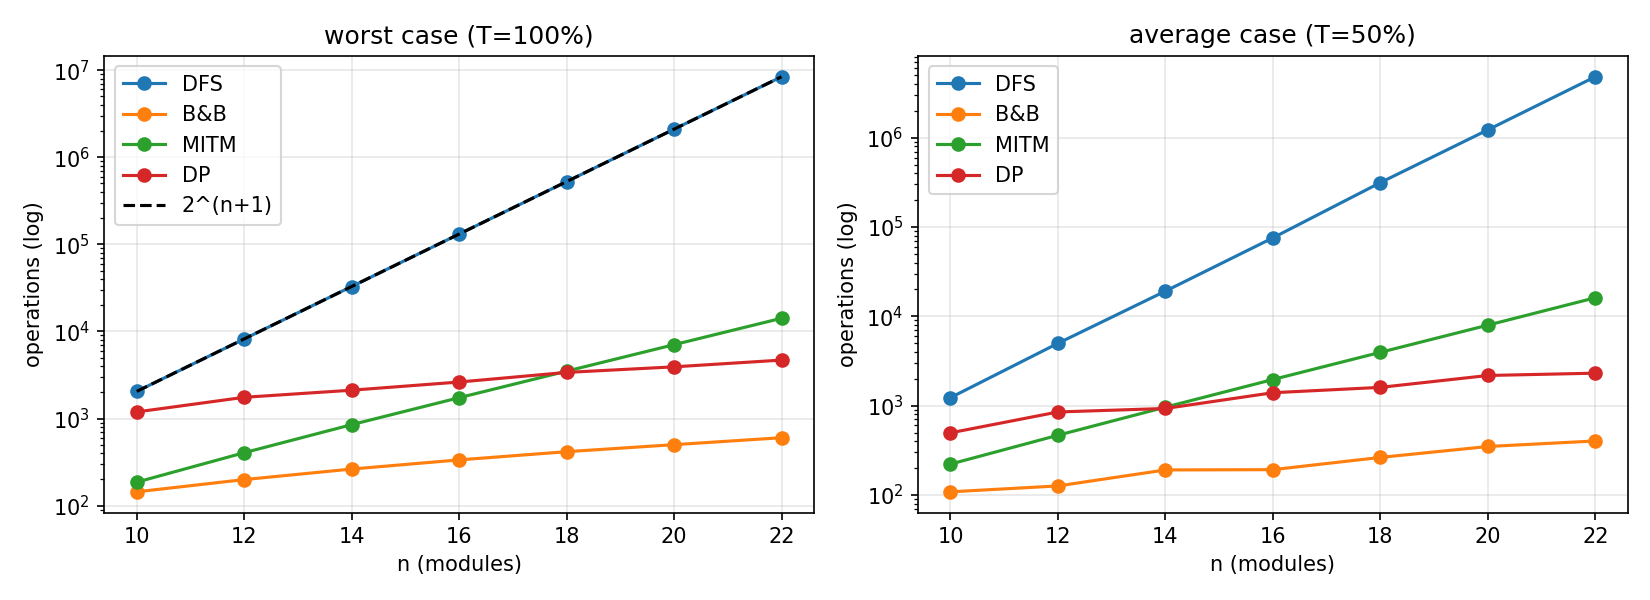
\includegraphics[width=\linewidth]{figures/fig_operations_vs_n.png}
\caption{Operations versus $n$ (log scale). The DFS follows $2^{n+1}-1$ in the worst case (left) and has the same exponential trend in the average case (right); DP, Branch and Bound and Meet-in-the-Middle grow much more slowly in this range.}\label{fig:ops-vs-n}
\end{figure}

\begin{figure}[h]
\centering
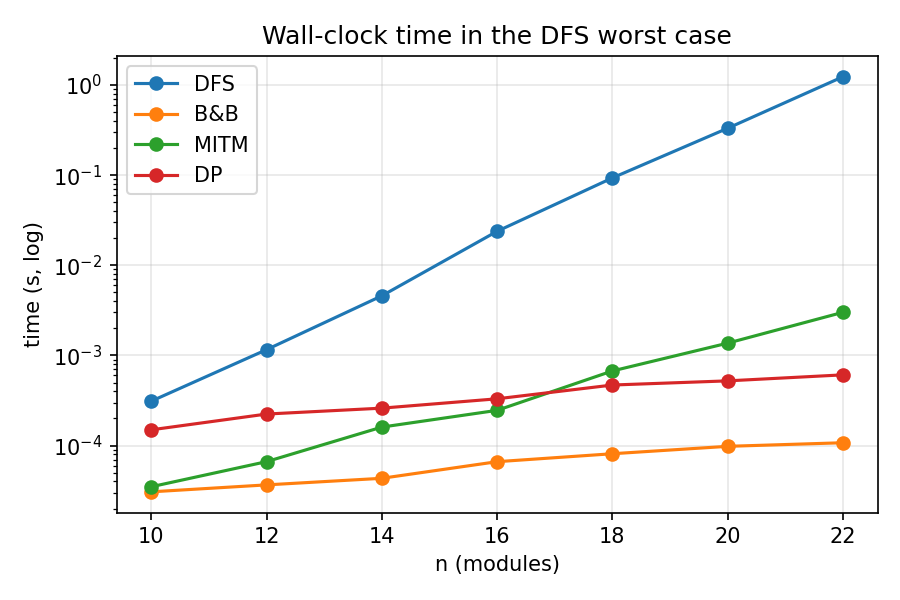
\includegraphics[width=0.62\linewidth]{figures/fig_time_vs_n.png}
\caption{Wall-clock time versus $n$ in the DFS worst case (log scale).}\label{fig:time-vs-n}
\end{figure}

In this range the DP is comparatively expensive in operations for small $n$ (its cost is $n(T+1)$ regardless of the data), while Branch and Bound needs very few operations: even in the DFS worst case it performs only 602 operations at $n=22$, because when every module fits the greedy path is optimal and the bound prunes everything else. This scenario is therefore favorable to Branch and Bound; Section~\ref{sec:exp-families} shows that this does not hold for all instance families.

\subsection{Dynamic programming and greedy at scale}

The DFS cannot be run at large $n$, but the DP and the greedy can. Table~\ref{tab:scale} and Figure~\ref{fig:scale} report $n$ from 50 to 600 modules (uncorrelated family, $\rho=0.5$). The number of DP operations coincides \emph{exactly} with $n(T+1)$ at every size, confirming Theorem~\ref{thm:dp}. The DP solves an instance with 600 modules and $T=3{,}060$ time units in about 0.37~s of pure Python, i.e.\ roughly 0.2~$\mu$s per cell. The vector version is about 40\% faster because it avoids allocating the table. The greedy performs between 0.95 and 0.98 operations per $n\log_2 n$, as expected from Proposition~\ref{prop:greedy-time}, and takes less than two milliseconds.

\begin{table}[h]
\centering
\caption{DP and greedy at scale (uncorrelated family, $R=20$, $\rho=0.5$).}\label{tab:scale}
\footnotesize\setlength{\tabcolsep}{4pt}
\begin{tabular}{@{}r r r r r r r r@{}}
\toprule
$n$ & $T$ & DP ops $=n(T+1)$ & DP time (s) & DP-vector (s) & Greedy ops & Greedy ops$/(n\log_2 n)$ & Greedy (s)\\
\midrule
50 & 273 & 13,700 & 0.0017 & 0.0010 & 269 & 0.95 & 0.0001\\
100 & 528 & 52,900 & 0.0081 & 0.0053 & 636 & 0.96 & 0.0002\\
200 & 1,097 & 219,600 & 0.0369 & 0.0247 & 1,486 & 0.97 & 0.0004\\
400 & 1,991 & 796,800 & 0.1396 & 0.0924 & 3,354 & 0.97 & 0.0011\\
600 & 3,060 & 1,836,600 & 0.3697 & 0.2230 & 5,400 & 0.98 & 0.0016\\
\bottomrule
\end{tabular}

\end{table}

\begin{figure}[h]
\centering
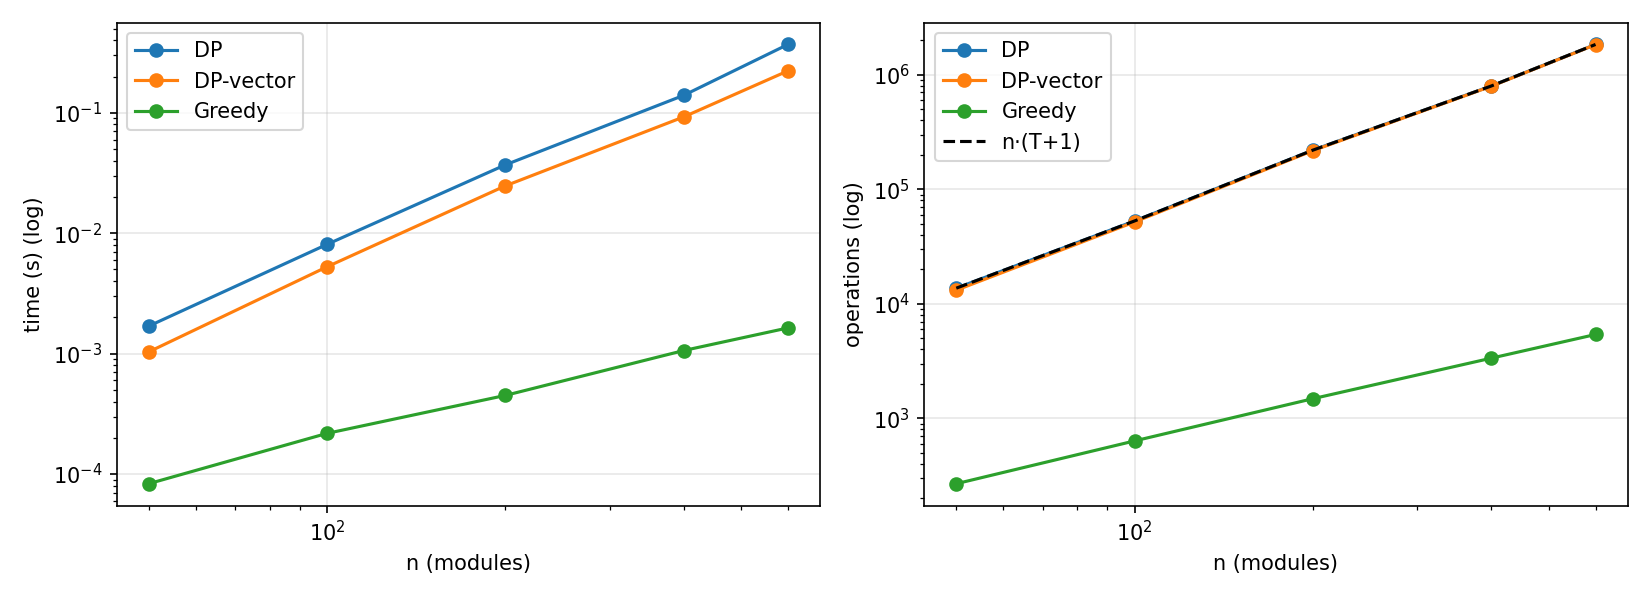
\includegraphics[width=\linewidth]{figures/fig_scale.png}
\caption{Time and operations of the DP and the greedy as $n$ grows (log--log). The dashed line is $n(T+1)$, which the DP operation count matches exactly.}\label{fig:scale}
\end{figure}

\subsection{Pseudo-polynomial behavior}

To demonstrate Proposition~\ref{prop:pseudo} we keep the same 18 modules and multiply all times and the budget by a factor from 1 to 1,024 (for instance, hours expressed in minutes and then in smaller units). The structure of the instance does not change, only the \emph{magnitude} of $T$, which goes from 100 to 102,400. Table~\ref{tab:pseudo} and Figure~\ref{fig:pseudo} show that the DP operations grow in proportion to $T$ (from 1,818 to 1,843,218, a factor of about 1,014 for a factor of 1,024 in $T$) and its time from 0.0002~s to 0.27~s, whereas the DFS, Branch and Bound, Meet-in-the-Middle and greedy counts do not change at all: they depend on $n$ and not on $T$.

\begin{table}[h]
\centering
\caption{Effect of the magnitude of $T$ ($n=18$ fixed; times and budget multiplied by the factor).}\label{tab:pseudo}
\small
\begin{tabular}{@{}r r r r r r r r@{}}
\toprule
Factor & $T$ & DP ops & DP time (s) & DFS ops & B\&B ops & MITM ops & Greedy ops\\
\midrule
$\times1$ & 100 & 1,818 & 0.0002 & 313,216 & 265 & 4,005 & 74\\
$\times4$ & 400 & 7,218 & 0.0009 & 313,216 & 265 & 4,005 & 74\\
$\times16$ & 1,600 & 28,818 & 0.0038 & 313,216 & 265 & 4,005 & 74\\
$\times64$ & 6,400 & 115,218 & 0.0153 & 313,216 & 265 & 4,005 & 74\\
$\times256$ & 25,600 & 460,818 & 0.0662 & 313,216 & 265 & 4,005 & 74\\
$\times1024$ & 102,400 & 1,843,218 & 0.2657 & 313,216 & 265 & 4,005 & 74\\
\bottomrule
\end{tabular}

\end{table}

\begin{figure}[h]
\centering
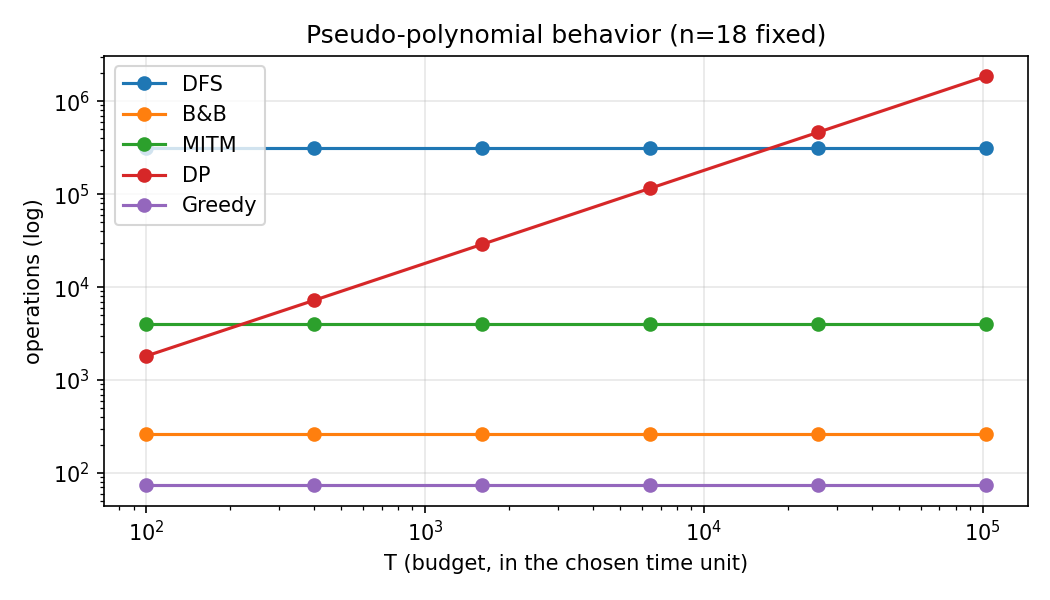
\includegraphics[width=0.75\linewidth]{figures/fig_pseudopolynomial.png}
\caption{Operations versus $T$ for fixed $n=18$ (log--log). Only the DP grows with $T$.}\label{fig:pseudo}
\end{figure}

\subsection{Quality of the greedy heuristic}\label{sec:exp-greedy}

Table~\ref{tab:quality} reports the mean and the worst gap of the greedy and of the greedy with the best single module over 30 instances per cell, for $\rho=0.3$; Figure~\ref{fig:quality} shows the gap as a function of the budget and of $n$.

\begin{table}[h]
\centering
\caption{Gap with respect to the optimum, $\rho=0.3$ (30 instances per row, $R=20$).}\label{tab:quality}
\small
\begin{tabular}{@{}r l r r r r@{}}
\toprule
$n$ & Family & Greedy mean gap & Greedy max gap & Greedy+item mean & Greedy+item max\\
\midrule
8 & Uncorrelated & 1.8\% & 10.8\% & 1.8\% & 10.8\%\\
8 & Weakly corr. & 5.5\% & 25.9\% & 5.4\% & 24.0\%\\
8 & Strongly corr. & 7.0\% & 19.0\% & 7.0\% & 19.0\%\\
\midrule
15 & Uncorrelated & 1.7\% & 9.1\% & 1.7\% & 9.1\%\\
15 & Weakly corr. & 2.7\% & 8.9\% & 2.7\% & 8.9\%\\
15 & Strongly corr. & 3.2\% & 7.9\% & 3.2\% & 7.9\%\\
\midrule
30 & Uncorrelated & 0.4\% & 2.8\% & 0.4\% & 2.8\%\\
30 & Weakly corr. & 1.0\% & 3.6\% & 1.0\% & 3.6\%\\
30 & Strongly corr. & 2.2\% & 4.6\% & 2.2\% & 4.6\%\\
\midrule
60 & Uncorrelated & 0.5\% & 1.8\% & 0.5\% & 1.8\%\\
60 & Weakly corr. & 0.2\% & 0.9\% & 0.2\% & 0.9\%\\
60 & Strongly corr. & 0.8\% & 2.2\% & 0.8\% & 2.2\%\\
\bottomrule
\end{tabular}

\end{table}

\begin{figure}[h]
\centering
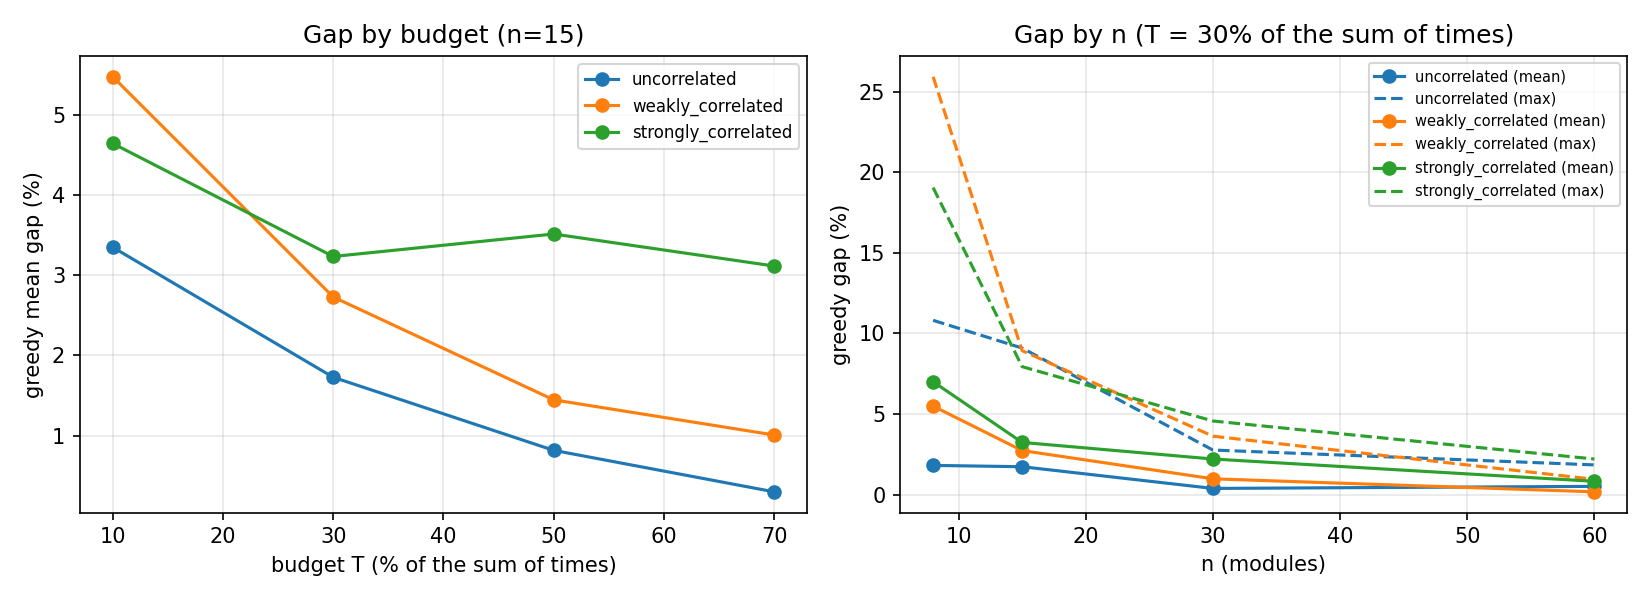
\includegraphics[width=\linewidth]{figures/fig_greedy_quality.png}
\caption{Mean gap of the greedy by budget ratio ($n=15$, left) and mean and maximum gap by $n$ ($\rho=0.3$, right).}\label{fig:quality}
\end{figure}

Three observations follow. First, the \emph{mean} gap is small and decreases with $n$: with many modules that are small relative to the budget, the greedy is nearly optimal (for instance, 0.8\% on the strongly correlated family at $n=60$). Second, the \emph{worst} gap is much larger, especially with few modules (25.9\% at $n=8$ for $\rho=0.3$, and 54.5\% at $\rho=0.1$, Table~\ref{tab:quality-item}), and it reaches 99.8\% on the adversarial instance of Section~\ref{sec:testinstance}: a small average gap offers no guarantee. Third, at $\rho=0.3$ the strongly correlated family yields the largest mean gap for every $n$ tested, in agreement with the intuition that short modules with high ratio block longer modules that are worth more; the ordering is not universal, though (at $\rho=0.1$ and $n=15$ the weakly correlated family is slightly worse, 5.5\% against 4.6\%).

\begin{table}[h]
\centering
\caption{Effect of adding the best single module to the greedy, $\rho=0.1$ (30 instances per row).}\label{tab:quality-item}
\small
\begin{tabular}{@{}r l r r r r@{}}
\toprule
$n$ & Family & Greedy mean gap & Greedy max gap & Greedy+item mean & Greedy+item max\\
\midrule
8 & Uncorrelated & 2.5\% & 50.0\% & 0.0\% & 0.0\%\\
8 & Weakly corr. & 6.7\% & 54.5\% & 0.8\% & 12.5\%\\
8 & Strongly corr. & 7.1\% & 35.0\% & 1.1\% & 11.1\%\\
\midrule
15 & Uncorrelated & 3.4\% & 23.1\% & 3.4\% & 23.1\%\\
15 & Weakly corr. & 5.5\% & 19.0\% & 5.0\% & 19.0\%\\
15 & Strongly corr. & 4.6\% & 14.6\% & 4.6\% & 14.6\%\\
\bottomrule
\end{tabular}

\end{table}

Table~\ref{tab:quality-item} shows what the variant of Proposition~\ref{prop:greedy-half} does in practice. With tight budgets and few modules, where a single module nearly fills the knapsack, it repairs the worst cases (for $n=8$, the mean gap on the weakly correlated family falls from 6.7\% to 0.8\% and the worst gap from 54.5\% to 12.5\%). For $n=15$ it brings practically no improvement, and at $\rho=0.3$ almost none for any $n$ tested (Table~\ref{tab:quality}), so the main benefit of the variant is the guarantee, not the average quality.

\subsection{Exact algorithms across instance families}\label{sec:exp-families}

Table~\ref{tab:families} and Figure~\ref{fig:families} compare Branch and Bound, Meet-in-the-Middle and the DP on uncorrelated and strongly correlated instances with $R=1000$ (so that the budget is large, which is the regime in which the DP is most expensive), $\rho=0.5$, five instances per row.

\begin{table}[h]
\centering
\caption{Operations of the exact algorithms by family ($R=1000$, $\rho=0.5$, 5 instances per row).}\label{tab:families}
\small
\begin{tabular}{@{}l r r r r r@{}}
\toprule
Family & $n$ & B\&B mean & B\&B max & MITM & DP\\
\midrule
Uncorrelated & 20 & 428 & 690 & 8,028 & 95,070\\
Uncorrelated & 30 & 683 & 834 & 261,460 & 211,032\\
Uncorrelated & 40 & 1,377 & 2,087 & 8,387,202 & 389,768\\
\midrule
Strongly corr. & 20 & 6,596 & 26,368 & 8,028 & 95,070\\
Strongly corr. & 30 & 7,655 & 16,935 & 261,460 & 211,032\\
Strongly corr. & 40 & 17,162 & 44,475 & 8,387,202 & 389,768\\
\bottomrule
\end{tabular}

\end{table}

\begin{figure}[h]
\centering
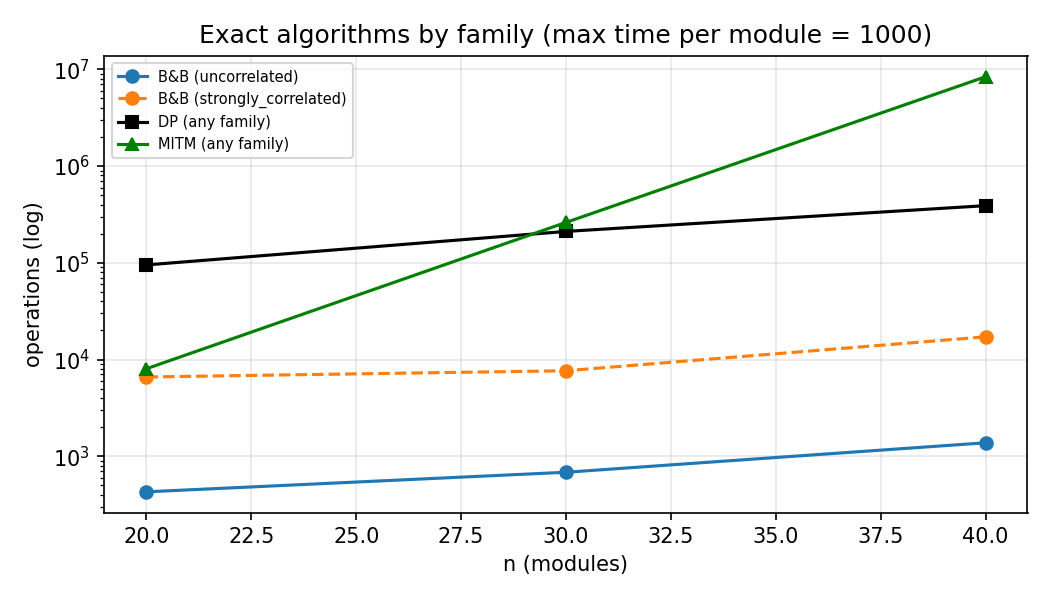
\includegraphics[width=0.75\linewidth]{figures/fig_exact_by_family.png}
\caption{Mean operations by $n$ for Branch and Bound on two families, compared with the DP and Meet-in-the-Middle (which do not depend on the family).}\label{fig:families}
\end{figure}

DP and Meet-in-the-Middle cost the same in both families, as predicted: their cost depends on $n$ and $T$ (DP) or on $n$ (MITM), not on the relation between times and scores. Branch and Bound, in contrast, depends strongly on the family: on strongly correlated instances it needs 11 to 15 times more operations than on uncorrelated ones (for instance 17,162 against 1,377 on average at $n=40$), and its worst observed run (44,475 operations) is 21 times its worst uncorrelated run (2,087). This agrees with the literature, where strongly correlated instances are reported as hard for branch-and-bound algorithms \cite{pisinger2005}; a plausible explanation, which we did not test, is that the fractional bound is less effective on them. Meet-in-the-Middle grows by a factor of 32 from $n=30$ to $n=40$ (261,460 to 8,387,202), exactly the factor $2^{10/2}$ predicted by Theorem~\ref{thm:mitm}, and from $n=30$ on it already costs more than the DP (21.5 times more at $n=40$) because $T$ is small relative to $2^{n/2}$.

\subsection{FPTAS}

Table~\ref{tab:fptas} compares the FPTAS with the exact DP on a strongly correlated instance with $n=30$.

\begin{table}[h]
\centering
\caption{FPTAS versus exact DP ($n=30$, strongly correlated, $R=20$, $\rho=0.5$).}\label{tab:fptas}
\small
\begin{tabular}{@{}l r r r r@{}}
\toprule
Algorithm & $\varepsilon$ & Score & Score / optimum & Operations\\
\midrule
exact DP & --- & 365 & 1.0000 & 4,680\\
FPTAS & 0.5 & 365 & 1.0000 & 36,690\\
FPTAS & 0.2 & 365 & 1.0000 & 91,680\\
FPTAS & 0.1 & 365 & 1.0000 & 183,330\\
FPTAS & 0.05 & 365 & 1.0000 & 366,630\\
\bottomrule
\end{tabular}

\end{table}

The FPTAS reaches the optimum in every case (ratio 1.0000, far better than the guaranteed $1-\varepsilon$), but at a high cost: it performs 7.8 times more operations than the exact DP with $\varepsilon=0.5$ and 78 times more with $\varepsilon=0.05$. The operation count grows in proportion to $1/\varepsilon$ (a factor of about 2.5, 2.0 and 2.0 as $\varepsilon$ goes from 0.5 to 0.2, 0.1 and 0.05), in agreement with Theorem~\ref{thm:fptas}. With a small $T$, approximating is more expensive than solving exactly; the FPTAS pays off only when $T$ is so large that $n(T+1)$ exceeds $n^3/\varepsilon$.

\subsection{The article's DFS on a prerequisite graph}\label{sec:exp-graph}

Finally, \code{dfs\_paths} was executed on a complete DAG (an edge from $i$ to every $j>i$), the worst case for the strategy of the article. Table~\ref{tab:graph} shows that the number of generated paths is exactly $2^{n-1}$ for every $n$ tested (32,768 paths for $n=16$), as derived in Section~\ref{sec:design}: the exhaustive path enumeration of the article is exponential in the size of the course graph.

\begin{table}[h]
\centering
\caption{Paths generated by the prerequisite-graph DFS on a complete DAG.}\label{tab:graph}
\small
\begin{tabular}{@{}r rrrrrrr@{}}
\toprule
$n$ & 4 & 6 & 8 & 10 & 12 & 14 & 16\\
\midrule
Paths generated & 8 & 32 & 128 & 512 & 2,048 & 8,192 & 32,768\\
$2^{n-1}$ & 8 & 32 & 128 & 512 & 2,048 & 8,192 & 32,768\\
\bottomrule
\end{tabular}

\end{table}

\section{Discussion}\label{sec:discussion}

\subsection{Which algorithm is the most suitable for learning-path selection?}

Our analysis and experiments support the choice of \textbf{dynamic programming} as the most suitable algorithm for this scenario, for six reasons.

\begin{enumerate}[leftmargin=1.6em,itemsep=3pt]
\item \textbf{The answer must be optimal.} A recommendation that wastes part of the learner's time is a poor recommendation. The greedy lost up to 54.5\% of the score on small random instances, 15.4\% on the test instance and 99.8\% on the adversarial instance (Section~\ref{sec:exp-greedy}); the DP never loses anything (Lemma~\ref{lem:rec}).
\item \textbf{The parameter that makes the DP expensive is small in this domain.} The study load of a learner is expressed in minutes or blocks of a few minutes, so $T$ stays in the low thousands. With 600 modules and $T=3{,}060$ the DP took 0.37~s in pure Python (Table~\ref{tab:scale}). The pseudo-polynomial nature (Proposition~\ref{prop:pseudo}) becomes a problem only if time is measured in very fine units, as in the experiment of $T\approx10^5$, where the cost reaches $1.8\times10^6$ operations for just 18 modules.
\item \textbf{The cost is predictable.} The DP performs exactly $n(T+1)$ operations on every instance (Theorem~\ref{thm:dp}), whereas Branch and Bound varied between 1,377 and 44,475 operations at the same $n$ depending on the family (Table~\ref{tab:families}). For a system that answers learners interactively, a worst-case guarantee is worth more than a better average.
\item \textbf{Realistic data are correlated.} Longer modules plausibly carry more content and a higher score. The strongly correlated family is exactly where the greedy loses the most on average and where Branch and Bound becomes 11 to 15 times more expensive, while the DP is unaffected.
\item \textbf{One table answers every budget.} Since $D[i][t]$ is defined for \emph{at most} $t$ time units, the last row gives the optimal score for any study load up to $T$, and the reconstruction works for each of them. No other algorithm studied provides this without being run again, and it answers the natural question ``what if I only had eight hours?''.
\item \textbf{It is simple to prove, to explain and to extend.} The optimal substructure is short (Lemma~\ref{lem:rec}), the table is visual, and the reconstruction explains why each module was selected, which is valuable in an educational recommender.
\end{enumerate}

\subsection{When another algorithm wins}

The DP is not the best algorithm in every regime, and the experiments show it. Table~\ref{tab:decision} summarizes which algorithm to choose depending on the situation.

\begin{table}[h]
\centering
\caption{Choice of algorithm by regime.}\label{tab:decision}
\small
\begin{tabularx}{\linewidth}{@{}X X@{}}
\toprule
Situation & Most suitable algorithm\\
\midrule
Small integer $T$ (minutes or hours), $n$ up to thousands, an exact answer and a guarantee are required & Dynamic programming\\
Immediate answer, many modules that are small relative to $T$, a loss of 1 to 3\% is acceptable & Greedy (preferably with the best single module, which provides the 1/2 guarantee)\\
Time measured in very fine units ($T$ in the millions) and $n$ up to about 40 & Meet-in-the-Middle, whose cost does not depend on $T$\\
Both $n$ and $T$ enormous and an error $\varepsilon$ is tolerated & FPTAS (in theory; at our scales it did not pay off)\\
Easy instances and moderate $n$, average speed matters more than a worst-case guarantee & Branch and Bound (in our tests it needed fewer operations than the DP for $n\le40$)\\
Prerequisites between modules (graph) & Path enumeration as in the article, or integer programming; tree-shaped precedence admits specific DPs; on general DAGs the problem is NP-hard \cite{samphaiboon2000}\\
\bottomrule
\end{tabularx}
\end{table}

A point that deserves honesty: in our experiments Branch and Bound performed fewer operations than the DP for every instance size tested ($n\le40$), even on strongly correlated instances. We nevertheless consider the DP more suitable because Branch and Bound offers no polynomial guarantee, its cost fluctuates strongly with the data (and the literature reports instances on which it explodes \cite{pisinger2005}), and our largest instances have only 40 modules. If an application is known to produce easy instances with moderate $n$, Branch and Bound is a legitimate choice.

\subsection{Agreement with the literature}

The experiments reproduce, on our implementation, the main statements of the theory presented in Section~\ref{sec:background}:
\begin{itemize}[leftmargin=1.4em,itemsep=2pt]
\item The DP is pseudo-polynomial: its operation count is exactly $n(T+1)$ and grows with the magnitude of $T$ alone \cite{garey1979,kellerer2004}.
\item Meet-in-the-Middle grows as $2^{n/2}$ and does not depend on $T$ \cite{horowitz1974}.
\item Strongly correlated instances are harder for branch-and-bound algorithms, while DP is insensitive to the correlation \cite{pisinger2005}.
\item The ratio-based greedy has no constant guarantee, but the variant with the best single module guarantees one half of the optimum \cite{kellerer2004}; the FPTAS cost grows with $1/\varepsilon$ \cite{ibarra1975,lawler1979}.
\item The exhaustive search of the article is exponential in the size of the graph (Section~\ref{sec:exp-graph}), which explains why a reasonable system either limits the size of the course graph or uses a more elaborate method \cite{nabizadeh2017rutico}.
\end{itemize}

\subsection{Threats to validity}

\begin{itemize}[leftmargin=1.4em,itemsep=2pt]
\item \textbf{Synthetic instances.} Scores and times are generated by three families; no real course data were used. The conclusion about correlation rests on the hypothesis that longer modules score higher.
\item \textbf{Strongly correlated constant.} We use $R/2$ instead of the $R/10$ common in the literature (Section~\ref{sec:method}), which may exaggerate the greedy gap relative to standard benchmarks.
\item \textbf{Size of the instances.} The DFS was run up to $n=22$ and Branch and Bound and Meet-in-the-Middle up to $n=40$ (in the family experiment); results for larger $n$ rely on the theory and on extrapolation.
\item \textbf{Python and one machine.} Absolute times depend on the interpreter and hardware; conclusions rely on operation counters. The counters of different algorithms are not strictly commensurable (a node of Branch and Bound is more expensive than a cell of the DP), although we included the cost of the bound computation to reduce this bias.
\item \textbf{Few instances per point.} Averages use 5 to 30 instances per point, so small differences should not be over-interpreted.
\end{itemize}

\section{Members and Activities}\label{sec:members}

\begin{table}[h]
\centering
\caption{Activities carried out by each group member.}\label{tab:members}
\small
\begin{tabularx}{\linewidth}{@{}l X@{}}
\toprule
Member & Activities\\
\midrule
{[Member Name 1]} & Study of the article (RUTICO) and of the course graph; implementation of \code{dfs.py} and \code{graph\_dfs.py}; analysis of the DFS (Sections~\ref{sec:design-dfs} and~\ref{sec:exp-graph}).\\
{[Member Name 2]} & Design and implementation of the dynamic programming (\code{dp.py}); proofs of correctness and complexity of the DP (Section~\ref{sec:complexity}); test instance and DP table.\\
{[Member Name 3]} & Implementation of the greedy algorithm and of the sort (\code{greedy.py}, \code{sorting.py}); extra algorithms (\code{branch\_and\_bound.py}, \code{meet\_in\_the\_middle.py}, \code{fptas.py}); instance generators.\\
{[Member Name 4]} & Experimental routine (\code{experiment.py}), execution of the experiments and plots; writing and integration of the report.\\
\bottomrule
\end{tabularx}
\end{table}

All members reviewed the whole code and the whole report, and each one is able to explain every code segment and every complexity derivation in the presentation, as required by the assignment.

% INSTRUCTIONS FOR THE GROUP (not printed): replace the bracketed names and activities above with
% the real ones. If your course policy requires declaring the use of AI tools, add a sentence here.

\section{Conclusion}\label{sec:conclusion}

\paragraph{General comments.} We studied the selection of learning modules under a study-time budget, modeled as the 0/1 knapsack problem, starting from the article RUTICO, whose solution is an exhaustive DFS. We showed that dynamic programming is the same search with memoization: the decision tree has $2^n$ leaves but only $n(T+1)$ distinct states. We proved the correctness and the best-, worst- and space complexity of the DFS ($\Theta(n)$ to $\Theta(2^n)$ nodes, with exactly $2^{n+1}-1$ nodes when everything fits), of the DP ($\Theta(nT)$, pseudo-polynomial) and of the greedy ($\Theta(n\log n)$, without a constant guarantee unless the best single module is considered), and of three additional algorithms. The experiments, based on hardware-independent operation counters and validated on more than a thousand random instances, confirmed each of these results. The DP is the most suitable algorithm for the learning-path scenario because it is exact, has a cost that does not depend on the data, and the budget $T$ is small in practice; the experiments also showed regimes in which Branch and Bound, Meet-in-the-Middle or the greedy are preferable.

\paragraph{Main difficulties.}
\begin{itemize}[leftmargin=1.4em,itemsep=2pt]
\item \textbf{The article does not use dynamic programming.} The solution of the authors is a DFS, so we had to implement it and justify the DP through its relation to the DFS (memoization) rather than assume it.
\item \textbf{Bridging the article and the knapsack.} The article works on a graph with prerequisites; the knapsack ignores them. Deciding how to state this relaxation, and keeping a graph version (\code{graph\_dfs.py}) for the authors' setting, required care.
\item \textbf{Fair comparisons.} Comparing algorithms with different cost structures is delicate: a Branch and Bound node costs $\bigO(n)$ because of the bound, a DP cell costs $\bigO(1)$. We counted the bound steps explicitly and we did not rely on wall-clock time alone.
\item \textbf{Interpreting the greedy.} Its mean gap is small for large $n$ but its worst gap is large; reporting only the mean would have been misleading, and showing only the worst case would have been unfair. The families and the budget ratio were needed to tell the whole story.
\item \textbf{Exponential experiments.} The DFS cannot be run beyond about 22 modules in reasonable time, so growth beyond that point is established by proof and extrapolation, not by measurement.
\item \textbf{Implementation details.} Hand-writing the merge sort to keep $\Theta(n\log n)$ in every case, using integer arithmetic for ratio comparisons, and handling deep recursion in the memoized DP.
\end{itemize}

\paragraph{Limitations.} The relaxation without prerequisites, synthetic instances, a single machine and interpreter, and instance sizes up to $n=600$ (and $n=40$ for the exponential algorithms) bound the scope of the conclusions (Section~\ref{sec:discussion}).

\paragraph{Future work.} (i) Incorporate prerequisites: the precedence-constrained knapsack, starting from tree-shaped prerequisites, for which dynamic programming remains applicable. (ii) Several constraints at once (time and difficulty), i.e.\ a multidimensional knapsack, where the DP table acquires one dimension per constraint. (iii) Replace the synthetic scores by the time and score estimates of the article and real course data. (iv) Evaluate larger instances with a compiled implementation, and mixed strategies such as DP for the bulk of the budget and Branch and Bound for the remainder.


% ================================================================= REFERENCES
\clearpage
\addcontentsline{toc}{section}{References}
\begin{thebibliography}{99}\small

\bibitem{nabizadeh2017rutico} A.~H. Nabizadeh, A.~M. Jorge, and J.~P. Leal. RUTICO: Recommending Successful Learning Paths Under Time Constraints. In \emph{Adjunct Publication of the 25th Conference on User Modeling, Adaptation and Personalization (UMAP '17)}. ACM, 2017. DOI: 10.1145/3099023.3099035.

\bibitem{nabizadeh2020survey} A.~H. Nabizadeh, J.~P. Leal, H.~N. Rafsanjani, and R.~R. Shah. Learning path personalization and recommendation methods: A survey of the state-of-the-art. \emph{Expert Systems with Applications}, 159:113596, 2020. DOI: 10.1016/j.eswa.2020.113596.

\bibitem{samphaiboon2000} N.~Samphaiboon and T.~Yamada. Heuristic and exact algorithms for the precedence-constrained knapsack problem. \emph{Journal of Optimization Theory and Applications}, 105(3):659--676, 2000.

\bibitem{karp1972} R.~M. Karp. Reducibility among combinatorial problems. In R.~E. Miller and J.~W. Thatcher, editors, \emph{Complexity of Computer Computations}, pages 85--103. Plenum Press, 1972.

\bibitem{garey1979} M.~R. Garey and D.~S. Johnson. \emph{Computers and Intractability: A Guide to the Theory of NP-Completeness}. W.~H. Freeman, 1979.

\bibitem{bellman1957} R.~Bellman. \emph{Dynamic Programming}. Princeton University Press, 1957.

\bibitem{dantzig1957} G.~B. Dantzig. Discrete-variable extremum problems. \emph{Operations Research}, 5(2):266--288, 1957.

\bibitem{kellerer2004} H.~Kellerer, U.~Pferschy, and D.~Pisinger. \emph{Knapsack Problems}. Springer, 2004.

\bibitem{pisinger2005} D.~Pisinger. Where are the hard knapsack problems? \emph{Computers \& Operations Research}, 32(9):2271--2284, 2005.

\bibitem{horowitz1974} E.~Horowitz and S.~Sahni. Computing partitions with applications to the knapsack problem. \emph{Journal of the ACM}, 21(2):277--292, 1974.

\bibitem{ibarra1975} O.~H. Ibarra and C.~E. Kim. Fast approximation algorithms for the knapsack and sum of subset problems. \emph{Journal of the ACM}, 22(4):463--468, 1975.

\bibitem{lawler1979} E.~L. Lawler. Fast approximation algorithms for knapsack problems. \emph{Mathematics of Operations Research}, 4(4):339--356, 1979.

\bibitem{land1960} A.~H. Land and A.~G. Doig. An automatic method of solving discrete programming problems. \emph{Econometrica}, 28(3):497--520, 1960.

\bibitem{kolesar1967} P.~J. Kolesar. A branch and bound algorithm for the knapsack problem. \emph{Management Science}, 13(9):723--735, 1967.

\bibitem{golomb1965} S.~W. Golomb and L.~D. Baumert. Backtrack programming. \emph{Journal of the ACM}, 12(4):516--524, 1965.

\bibitem{tarjan1972} R.~E. Tarjan. Depth-first search and linear graph algorithms. \emph{SIAM Journal on Computing}, 1(2):146--160, 1972.

\bibitem{michie1968} D.~Michie. ``Memo'' functions and machine learning. \emph{Nature}, 218:19--22, 1968.

\bibitem{cormen2022} T.~H. Cormen, C.~E. Leiserson, R.~L. Rivest, and C.~Stein. \emph{Introduction to Algorithms}. MIT Press, 4th edition, 2022.

\bibitem{kleinberg2006} J.~Kleinberg and \'E.~Tardos. \emph{Algorithm Design}. Addison-Wesley, 2006.

\bibitem{knuth1998} D.~E. Knuth. \emph{The Art of Computer Programming, Volume 3: Sorting and Searching}. Addison-Wesley, 2nd edition, 1998.

\bibitem{vazirani2001} V.~V. Vazirani. \emph{Approximation Algorithms}. Springer, 2001.

\bibitem{williamson2011} D.~P. Williamson and D.~B. Shmoys. \emph{The Design of Approximation Algorithms}. Cambridge University Press, 2011.

\end{thebibliography}


\appendix
\section{Reproducing the Results}\label{app:run}

\paragraph{Requirements.} Python 3.10 or newer and matplotlib (only for the plots), on Linux:
\begin{verbatim}
pip install matplotlib
python experiment.py                      # all blocks, about 1 minute
python experiment.py --quick              # reduced version
python experiment.py --only demo correctness
\end{verbatim}
The output of a full run is stored in \code{results/full\_output.txt}; the plots and the CSV files used by this report are in \code{results/}. The tables of Section~\ref{sec:experiments} are regenerated from the CSV files with \code{python report/make\_tables.py}, and the report is compiled with \code{pdflatex report.tex} (twice).

\paragraph{Experiment blocks.} Table~\ref{tab:blocks} maps each block of \code{experiment.py} to its parameters, outputs and the section of this report that discusses it. The operation counts are identical in every run; wall-clock times vary with the machine.

\begin{table}[h]
\centering
\caption{Experiment blocks, parameters and outputs.}\label{tab:blocks}
\footnotesize
\begin{tabularx}{\linewidth}{@{}l X p{4.4cm} l@{}}
\toprule
Block & Parameters (full run) & Outputs & Section\\
\midrule
\code{demo} & Test instance, $T=10$; adversarial instance, $T=1000$ & standard output & \ref{sec:testinstance}\\
\code{correctness} & 1,200 random instances, $n\le16$, seed 2024, $R\in\{5,20\}$, $\rho\in\{0.1,\dots,1.0\}$ & standard output & 6.2\\
\code{time} & $n=10,12,\dots,22$; worst case: uncorrelated, $\rho=1.0$; average: 5 instances, $\rho=0.5$ & \code{exponential\_time.csv}, \code{fig\_operations\_vs\_n.png}, \code{fig\_time\_vs\_n.png} & \ref{sec:exp-dfs}\\
\code{scale} & $n\in\{50,100,200,400,600\}$, uncorrelated, $\rho=0.5$ & \code{scale.csv}, \code{fig\_scale.png} & 6.4\\
\code{quality} & $n\in\{8,15,30,60\}$, 30 instances per point, $\rho\in\{0.1,0.3,0.5,0.7\}$, three families & \code{greedy\_quality.csv}, \code{fig\_greedy\_quality.png} & \ref{sec:exp-greedy}\\
\code{pseudo} & $n=18$, factors $1,4,\dots,1024$, uncorrelated, $\rho=0.5$ & \code{pseudopolynomial.csv}, \code{fig\_pseudopolynomial.png} & 6.5\\
\code{families} & $n\in\{20,30,40\}$, 5 instances, $R=1000$, $\rho=0.5$, uncorrelated and strongly correlated & \code{exact\_by\_family.csv}, \code{fig\_exact\_by\_family.png} & \ref{sec:exp-families}\\
\code{fptas} & $n=30$, strongly correlated, $\varepsilon\in\{0.5,0.2,0.1,0.05\}$ & \code{fptas.csv} & 6.8\\
\code{graph} & complete DAG, $n=4,6,\dots,16$ & \code{graph\_dfs.csv} & \ref{sec:exp-graph}\\
\bottomrule
\end{tabularx}
\end{table}


\end{document}
